\documentclass{myBeamer}


\DeclareMathOperator{\Cov}{Cov}
\DeclareMathOperator{\Var}{Var}
\DeclareMathOperator{\E}{\mathbb{E}}
\DeclareMathOperator{\Proba}{\mathbb{P}}

\newcommand{\Covb}[2]{\ensuremath{\Cov\!\left[#1,#2\right]}}
\newcommand{\Eb}[1]{\ensuremath{\E\!\left[#1\right]}}
\newcommand{\Pb}[1]{\ensuremath{\Proba\!\left[#1\right]}}
\newcommand{\Varb}[1]{\ensuremath{\Var\!\left[#1\right]}}

% norm
%\newcommand{\norm}[1]{\| #1 \|}

\newcommand{\indep}{\rotatebox[origin=c]{90}{$\models$}}





\usepackage{mathptmx,amsmath,amssymb,graphicx,bibentry,bbm,babel,ragged2e}

\makeatletter


\renewcommand{\addlogo}{
	\hfill	
	
\includegraphics[height=.4cm]{figures/logos/iconOM.png}
	
\includegraphics[scale=1]{figures/logos/openmole_dark.png}
}


\newcommand{\noun}[1]{\textsc{#1}}
\newcommand{\jitem}[1]{\item \begin{justify} #1 \end{justify} \vfill{}}
%\newcommand{\sframe}[2]{\frame{\frametitle{#1}\addlogo #2}}

\newenvironment{centercolumns}{\begin{columns}[c]}{\end{columns}}
%\newenvironment{jitem}{\begin{justify}\begin{itemize}}{\end{itemize}\end{justify}}

%\usetheme{Warsaw}
%\setbeamertemplate{footline}[text line]{}
%\setbeamersize{text margin left=15pt,text margin right=15pt}
%\setbeamertemplate{headline}{}
%\setbeamertemplate{footline}[frame number]
%\setbeamertemplate{navigation symbols}{}

\usetheme{Darmstadt}
\setbeamertemplate{headline}{}
\setbeamertemplate{navigation symbols}{}
\setbeamercolor{palette quaternary}{fg=primaryDarkOM, bg=primaryGreenOM}


%\setbeamercovered{transparent}
%\setbeamercolor{structure}{fg=purple!50!blue, bg=purple!50!blue}

\@ifundefined{showcaptionsetup}{}{%
 \PassOptionsToPackage{caption=false}{subfig}}
\usepackage{subfig}

\usepackage[utf8]{inputenc}
%\usepackage[T1]{fontenc}


\usepackage{tikz}

\usepackage{multirow}

\usepackage{mdframed}

%\usepackage[usenames,dvipsnames]{pstricks}
%\usepackage{auto-pst-pdf}


%\usepackage[dvipsnames]{xcolor}

\usepackage{threeparttable}


\usepackage{listings}
\lstset{language=Java} 

\makeatother



\usepackage{pifont}
%\newcommand{\cmark}{\textcolor{green}\ding{51}}
%\newcommand{\xmark}{\textcolor{red}\ding{55}}
\newcommand{\cmark}{\ding{51}}
\newcommand{\xmark}{\ding{55}}


\title[A scala library for spatial sensitivity analysis]{A scala library for spatial sensitivity analysis}
\author[Raimbault, Perret and Reuillon]{J. Raimbault$^{1,2,3,\ast}$, J. Perret$^{4,2}$ and R. Reuillon$^{2,3}$\medskip\\
$^{1}$ Center for Advanced Spatial Analysis, UCL\\
$^{2}$ UPS CNRS 3611 ISC-PIF\\
$^{3}$ UMR CNRS 8504 G{\'e}ographie-cit{\'e}s\\
$^{4}$ LaSTIG STRUDEL, IGN, ENSG, Univ. Paris-Est\smallskip\\
$^{\ast}$ \texttt{juste.raimbault@polytechnique.edu}
}
\date{GISRUK 2020\\
July 21st, 2020}
\institute{

\includegraphics[scale=0.5]{figures/logos/iconOM.png}

\includegraphics[scale=2]{figures/logos/openmole.png}
}

\begin{document}



\begin{frame}[plain]
	\titlepage
\end{frame}

%\addtocounter{framenumber}{-1}



\section{Introduction}



\sframe{Modeling and simulation in geography}{

\begin{columns}

	\begin{column}{0.5\textwidth}
	\centering
	
	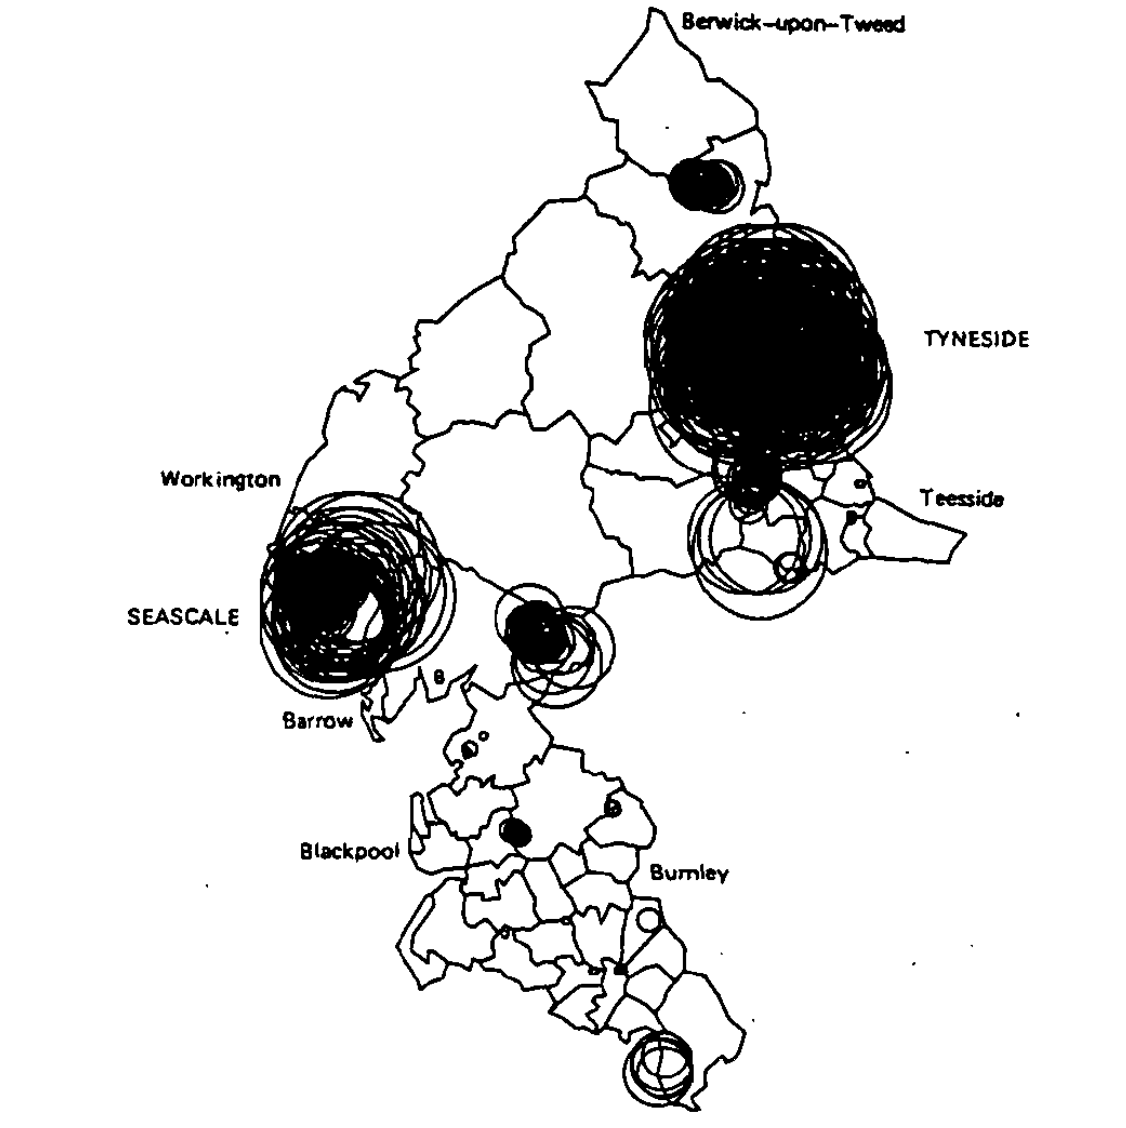
\includegraphics[width=0.6\textwidth]{figures/openshaw.png}
	
	\footnotesize
\textit{Geographical analysis machine \cite{openshaw1987mark}}
	
	\medskip
	\hrule
	\medskip
	
	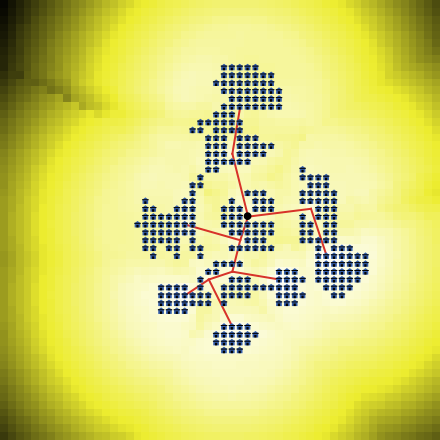
\includegraphics[width=0.55\textwidth,height=0.3\textheight]{figures/intro_RBD_lattice.png}
	
	\footnotesize
\textit{Hybrid urban morphogenesis \cite{raimbault2014hybrid}}
	

	\end{column}
	\vrule{}
	\begin{column}{0.5\textwidth}
	\centering
	
	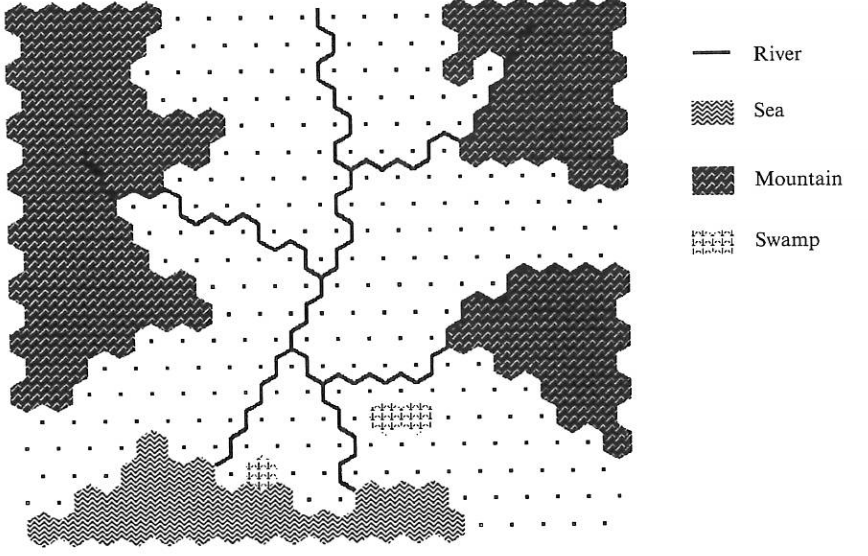
\includegraphics[width=0.7\textwidth]{figures/simpop1.png}
	
	\footnotesize
\textit{Simpop 1 model\cite{sanders1997simpop}}

	\medskip

	\hrule
	
	\medskip

	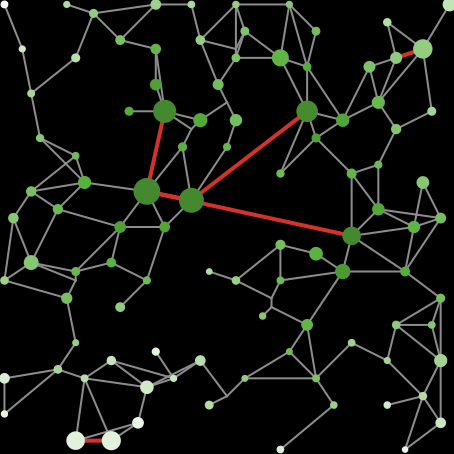
\includegraphics[width=0.6\textwidth]{figures/setup_synth_1_tick100.png}
	
	\footnotesize
	\textit{SimpopNet model \cite{schmitt2014modelisation}}
	
	\end{column}


\end{columns}

}




\sframe{Towards new practices: ERC Geodivercity}{

\begin{columns}
\begin{column}{0.4\textwidth}
	\centering
	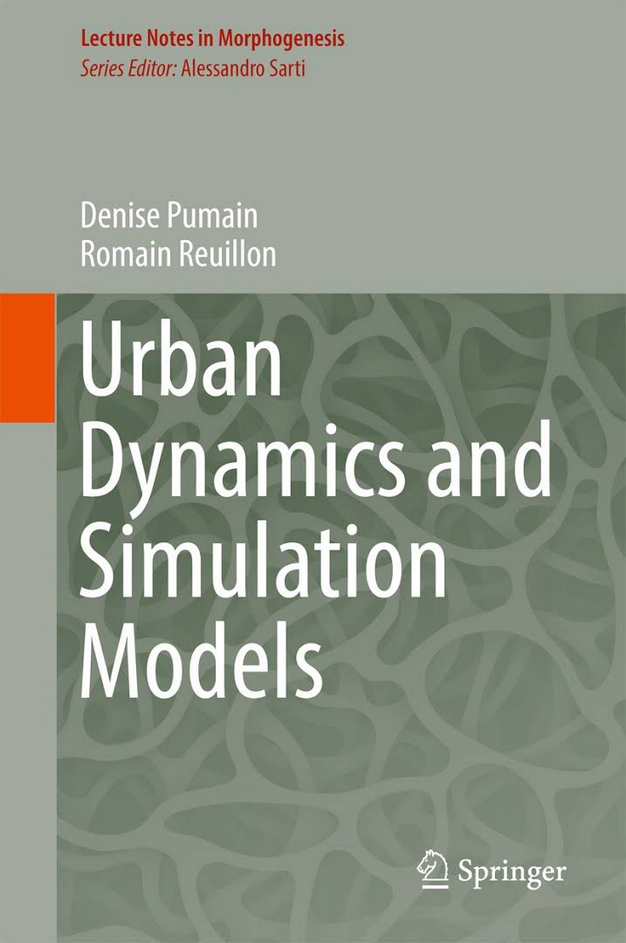
\includegraphics[width=\textwidth]{figures/urban-dynamics-simulation-models-geodivercity.png}
\end{column}
\begin{column}{0.6\textwidth}
	Development of an evolutionary urban theory \cite{pumain2018evolutionary}
	
	\medskip

	$\rightarrow$ Recurrent stylized facts on main systems of cities
	
	$\rightarrow$ Construction of simulation models (with an explicative purpose)
	
	$\rightarrow$ Tools and methods to explore simulation models
	
	\smallskip
	
	
\includegraphics[width=0.2\textwidth]{figures/logos/iconOM.png}
	
\includegraphics[width=0.7\textwidth]{figures/logos/openmole.png}
		
	
\end{column}
\end{columns}

}



\sframe{Sensitivity analysis issues in geography}{

\textit{Classical problems in geography and spatial sciences:}

\medskip

\begin{itemize}
	\item Modifiable Areal Unit Problem
	\item Dependancy of processes to scale
	\item Spatial non-stationarity
	\item Fuzzy and noisy data
	\item Genericity/particularity 
\end{itemize}

}


\sframe{The Modifiable Areal Unit Problem}{

\begin{center}
	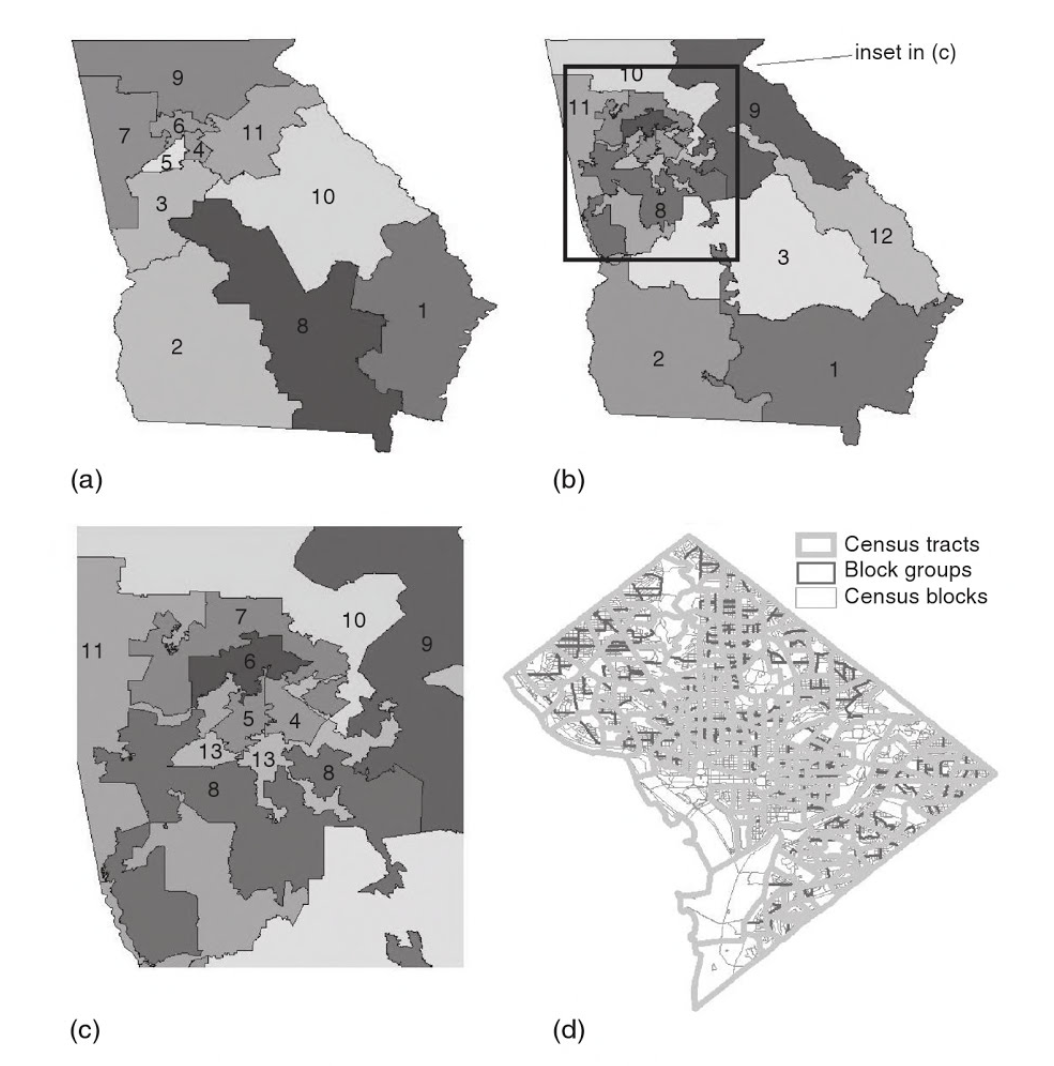
\includegraphics[height=0.75\textheight]{figures/maup.png}	
\end{center}


\medskip

\footnotesize

Wong, D. (2009). The modifiable areal unit problem (MAUP). The SAGE handbook of spatial analysis, 105, 23.

}


\sframe{Multiscalar systems}{

\textit{Processes specific to scales, coupling implies dedicated ontologies} \cite{raimbault:halshs-02351722}

\bigskip

\begin{center}
	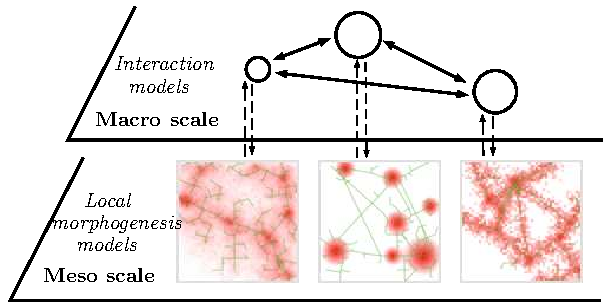
\includegraphics[width=0.9\textwidth]{figures/multiscale_morph.pdf}
\end{center}




}

\sframe{Spatial non-stationarity}{

\textit{Spatial non-stationarity of road network properties} \cite{raimbault2019urban}

\bigskip

\centering

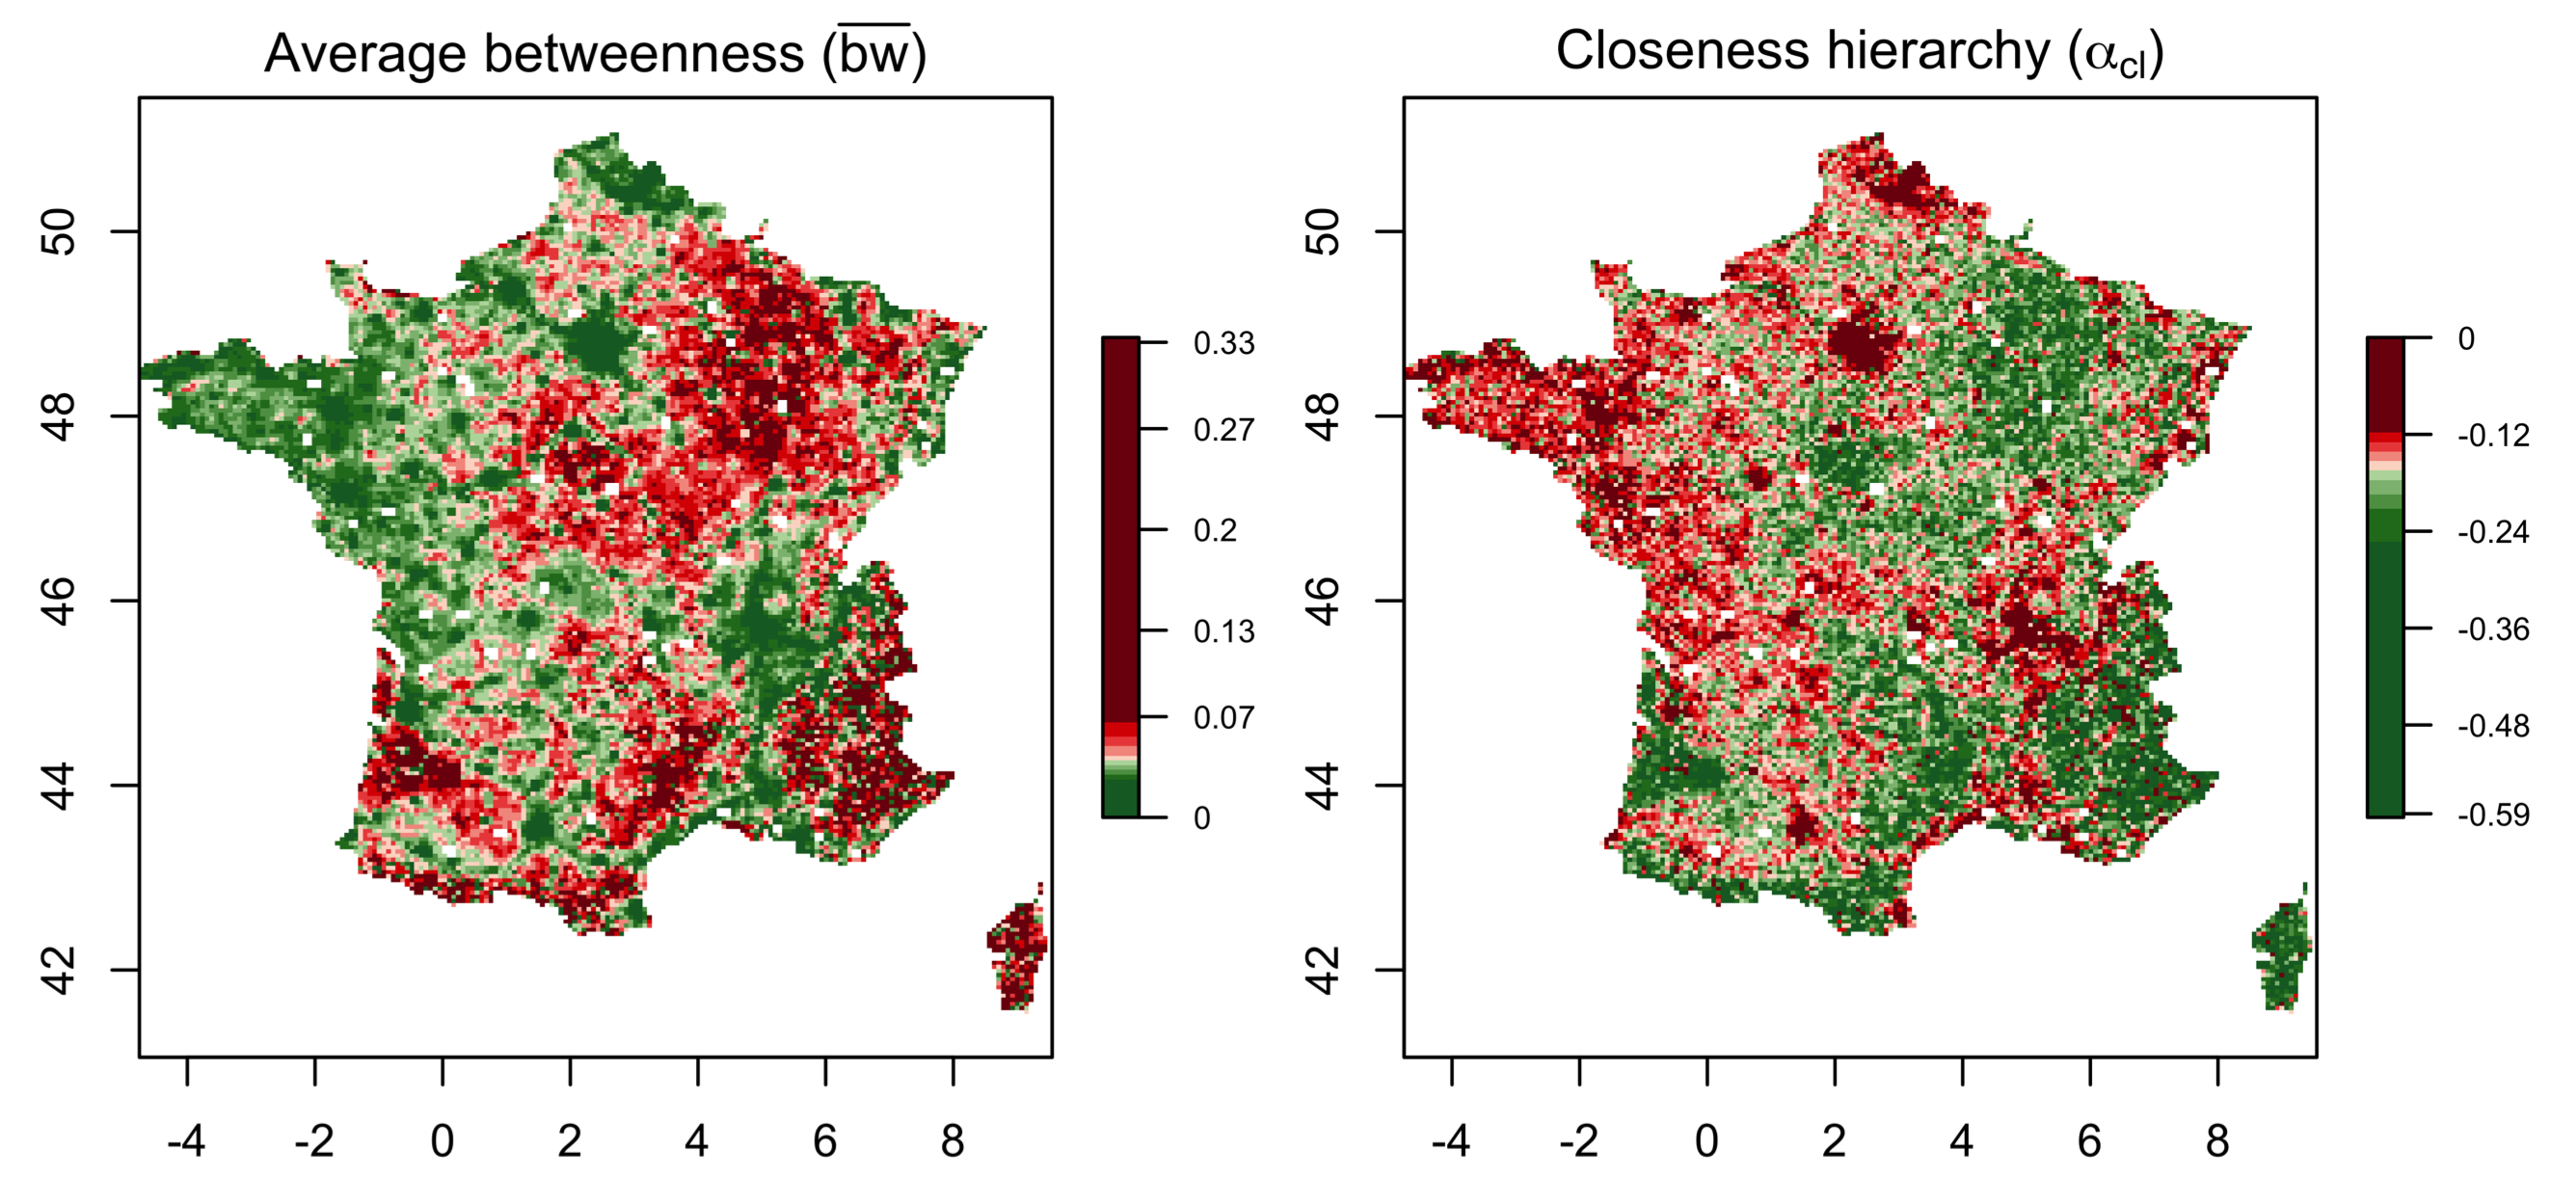
\includegraphics[width=\textwidth]{figures/nwindics_nonstat.png}

}


\sframe{Noisy spatial data}{

\textit{Assessment of data quality in OpenStreetMap} \cite{fan2014quality}

\medskip

\centering

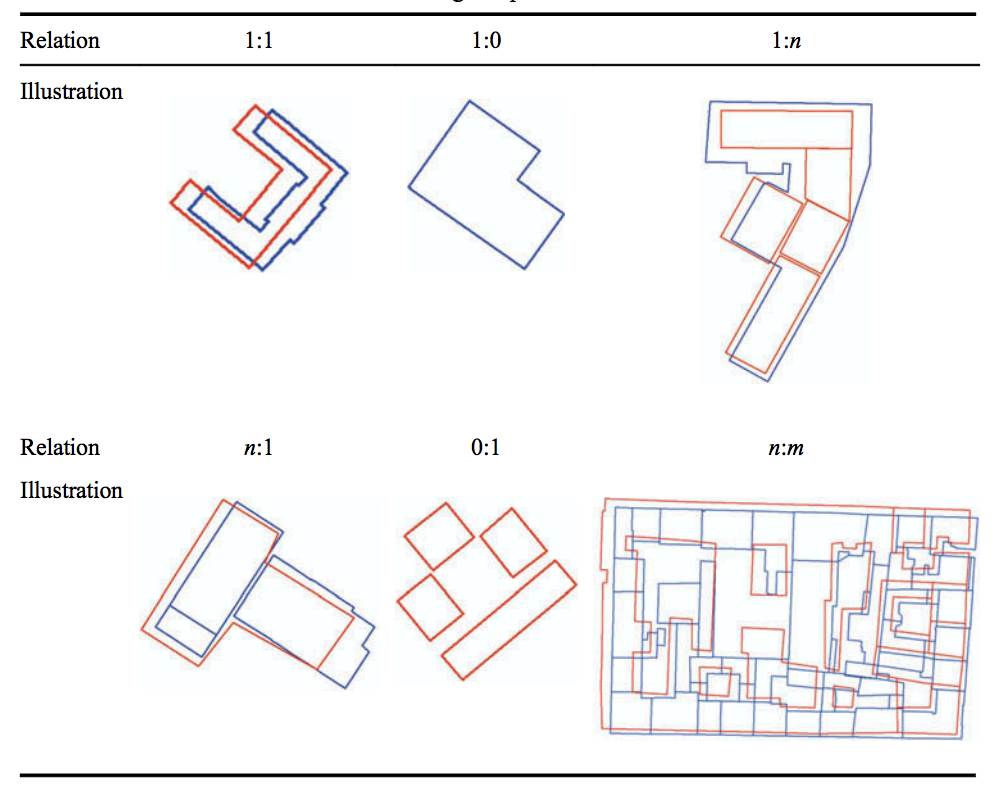
\includegraphics[height=0.8\textheight]{figures/osm_data_accuracy.png}

}


\sframe{Genericity and specificity}{

\textit{Urban systems are simultaneously universal and particular} \cite{raimbault2020empowering}

\medskip

\centering

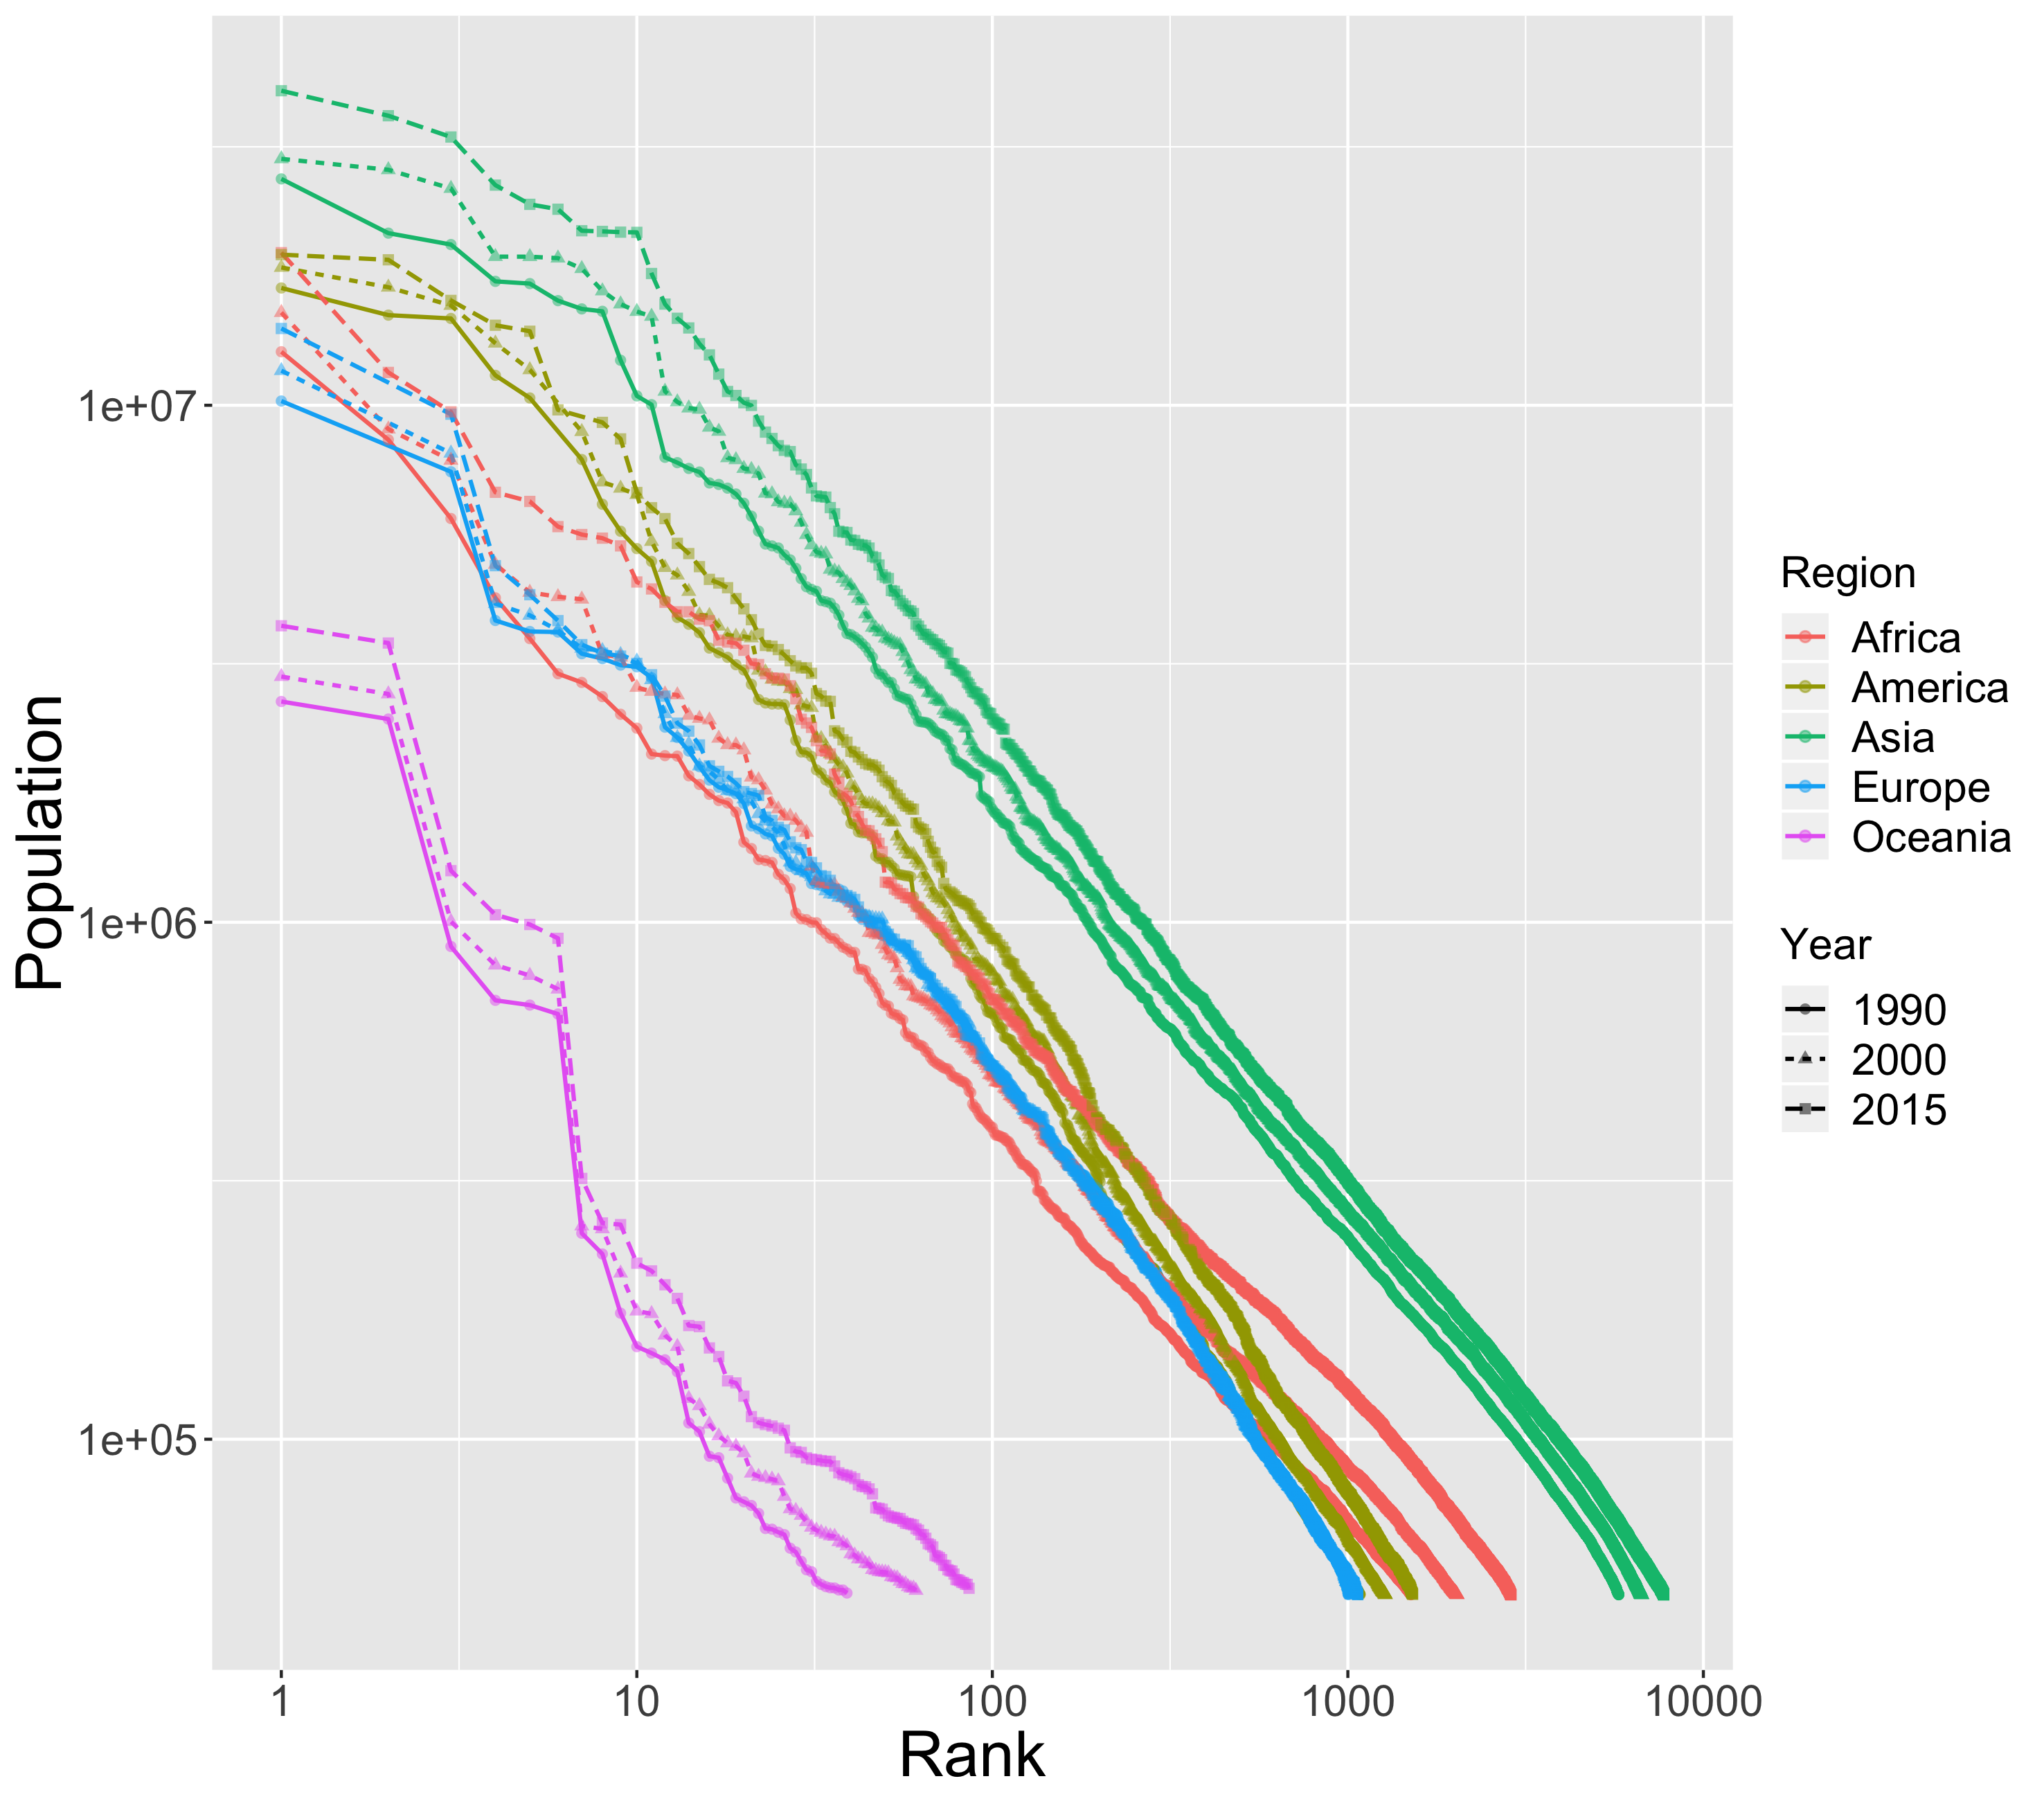
\includegraphics[height=0.8\textheight]{figures/zipf_sust.png}

}



\sframe{Approach proposed}{

$\implies$ \textbf{spatial configuration are parameters too}

\medskip

\begin{itemize}
	\item ``\textit{Space matters}'': impact of spatial configuration on model behavior
	\item Model behaviors which are robust to spatial configuration
	\item Model behaviors which are robust to noise in parametrization real datasets
\end{itemize}

 
}


\section{Spatial sensitivity methods}


\subsection{Spatial synthetic data}



\sframe{General context}{

\justify

$\rightarrow$ coupling models with spatial configuration generators (spatial synthetic data) gives model sensitivity to space through sensitivity analysis of the coupled model

\bigskip

$\rightarrow$ synthetic urban forms resembling real configurations

\bigskip

$\rightarrow$ at different scales: microscopic (buildings), mesoscopic (population distribution), macroscopic (system of cities)

}



\sframe{Generating building layouts}{

\textit{At the microscopic scale (district): generating building layouts}

\nocite{raimbault2019generating}

\medskip

Raimbault, J., \& Perret, J. (2019, July). Generating urban morphologies at large scales. In Artificial Life Conference Proceedings (pp. 179-186). MIT Press.

\medskip

\begin{itemize}
	\item systematic comparison of simple processual generators
	\item introduction of morphological indicators
	\item calibration on sampled layouts from OpenStreetMap
\end{itemize}

}


\sframe{Quantifying urban form}{

Urban form indicators for building layouts:

\medskip

\begin{itemize}
	\item density, number of buildings, average area
	\item Moran index and average distance on rasterized representation
	\item average detour in the free space
	\item mathematical morphology indicators (steps for erosion and dilation) \cite{serra1994morphological}
\end{itemize}


}


\sframe{Generators}{

\textit{Complementary generators}

\medskip

\begin{center}
	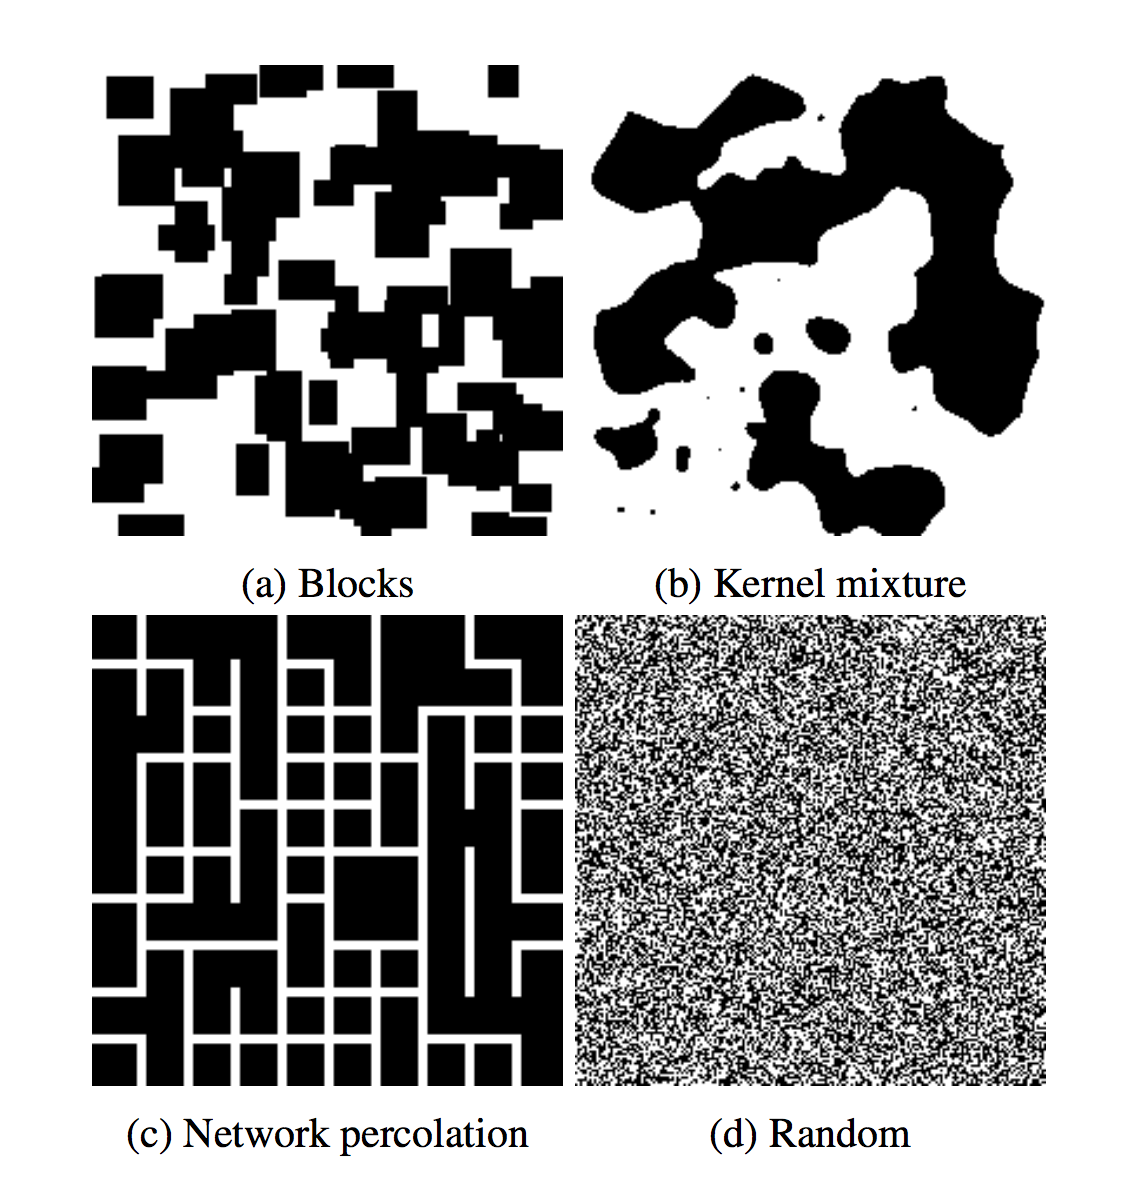
\includegraphics[height=0.85\textheight]{figures/spatialsens_examplegenerators.png}
\end{center}


}





\sframe{Synthetic population grids}{

\textit{At the mesoscopic scale: population grids}

\medskip


\begin{itemize}
	\item a reaction-diffusion model for population distributions
	\item urban form measures at the mesoscopic scale
	\item synthetic generators coupling population and road networks
\end{itemize}


\bigskip
\bigskip

\footnotesize

Raimbault, J. (2018). Calibration of a density-based model of urban morphogenesis. PloS one, 13(9), e0203516.

\nocite{raimbault2018calibration}

\smallskip

Raimbault, J. (2019). An urban morphogenesis model capturing interactions between networks and territories. In The Mathematics of Urban Morphology (pp. 383-409). Birkhäuser, Cham.

\nocite{raimbault2019urban}


}

\sframe{A simple Reaction-diffusion model}{


\justify

$\rightarrow$ Crucial role of the interplay between concentration forces and dispersion forces~\cite{fujita1996economics} in keeping Urban Systems at the border of chaos

\bigskip

$\rightarrow$ Potentiality of aggregation mechanisms (such as Simon model) to produce power laws

\bigskip

$\rightarrow$ Link with Reaction-diffusion approaches in Morphogenesis

\cite{turing1952chemical}

\bigskip

$\rightarrow$ Extension of a DLA-type model introduced by \cite{batty1991generating}, with simple abstract processes of population aggregation and diffusion

}


\sframe{Model Formalization}{

$\rightarrow$ Grid world with cell populations $(P_i(t))_{1\leq i\leq N^2}$.

\bigskip

$\rightarrow$ At each time step:

\begin{enumerate}
\item Population growth with exogenous rate $N_G$, attributed independently to a cell following a preferential attachment of strength $\alpha$
%\begin{equation}
%\Pb{P_i(t+1)=P_i(t)+1|P(t+1)=P(t)+1}=\frac{(P_i(t)/P(t))^{\alpha}}{\sum(P_i(t)/P(t))^{\alpha}}
%\end{equation}
%The attribution being uniformly drawn if all population are equal to 0.
\item Population is diffused $n_d$ times with strength $\beta$
\end{enumerate}

\bigskip

$\rightarrow$ Stopping criterion: fixed maximal population $P_m$.

%To avoid bord effects such as reflecting diffusion waves, border cells diffuse their due proportion outside of the world, implying that the total population at time $t$ is strictly smaller than $N_G\cdot t$.

\bigskip

$\rightarrow$ Output measured by morphological indicators: Moran index, average distance, rank-size hierarchy, entropy.


}


\sframe{Generating Population Distributions}{

\centering

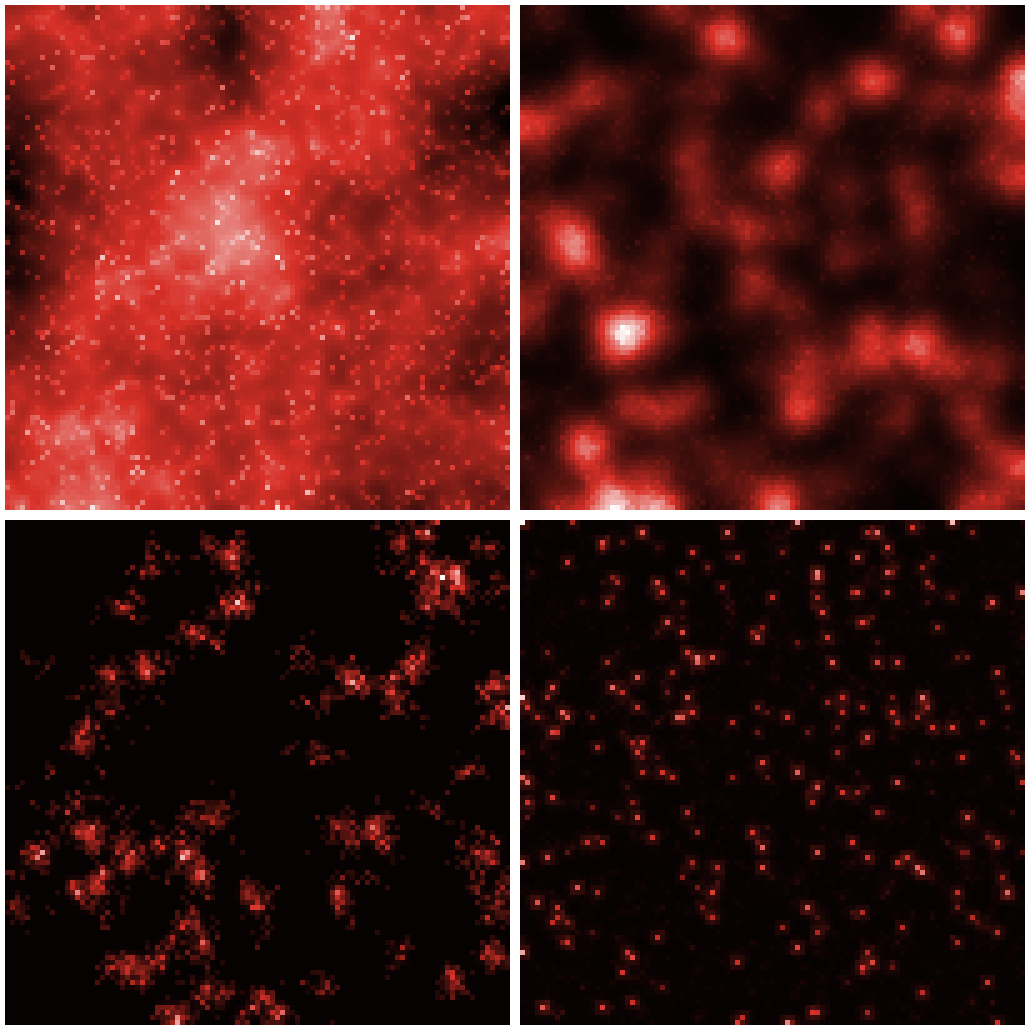
\includegraphics[height=0.8\textheight]{figures/density_Fig2}

\footnotesize\textit{Examples of generated territorial shapes}

}


\sframe{Morphological indicators}{

\begin{enumerate}
\item Rank-size slope $\gamma$, given by $\ln \left( P_{\tilde{i}}/P_0\right) \sim k + \gamma\cdot \ln \left(\tilde{i}/i_0\right)$ where $\tilde{i}$ are the indexes of the distribution sorted in decreasing order.
\item Entropy of the distribution:
\begin{equation}
\mathcal{E} = \sum_{i=1}^{M}\frac{P_i}{P}\cdot \ln{\frac{P_i}{P}}
\end{equation}
$\mathcal{E}=0$ means that all the population is in one cell whereas $\mathcal{E}=0$ means that the population is uniformly distributed.
\item Spatial-autocorrelation given by Moran index, with simple spatial weights given by $w_{ij} = 1/d_{ij}$
\[
I = M \cdot \frac{\sum_{i\neq j} w_{ij} \left(P_i - \bar{P}\right)\cdot\left(P_j - \bar{P}\right)}{\sum_{i\neq j} w_{ij} \sum_{i}{\left( P_i - \bar{P}\right)}^2}
\]
\item Mean distance between individuals
\[
\bar{d} = \frac{1}{d_M}\cdot \sum_{i<j} \frac{P_i P_j}{P^2} \cdot d_{ij}
\]
where $d_M$ is a normalisation constant
\end{enumerate}



}




\sframe{Network Generation models}{

\textit{currently being implemented}

\medskip

Network generated conditionally to population; at fixed time steps:

\begin{enumerate}
	\item Add new nodes preferentially to new population and connect them
	\item \justify Variable heuristic for new links, among: nothing, random, gravity-based deterministic breakdown, gravity-based random breakdown (from \cite{schmitt2014modelisation}), cost-benefits (from \cite{louf2013emergence}), biological network generation (based on \cite{tero2010rules})
\end{enumerate}

\medskip

\centering

\frame{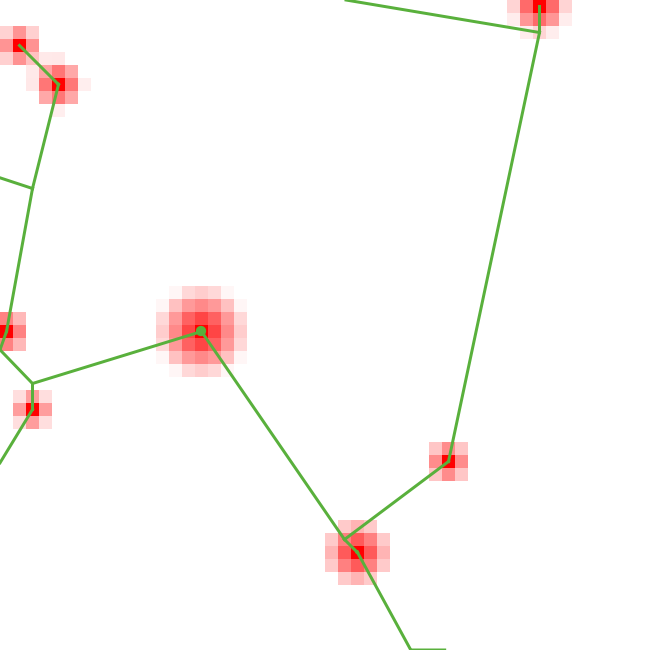
\includegraphics[width=0.32\textwidth]{figures/example_nwgrowth_tick0.png}}
\frame{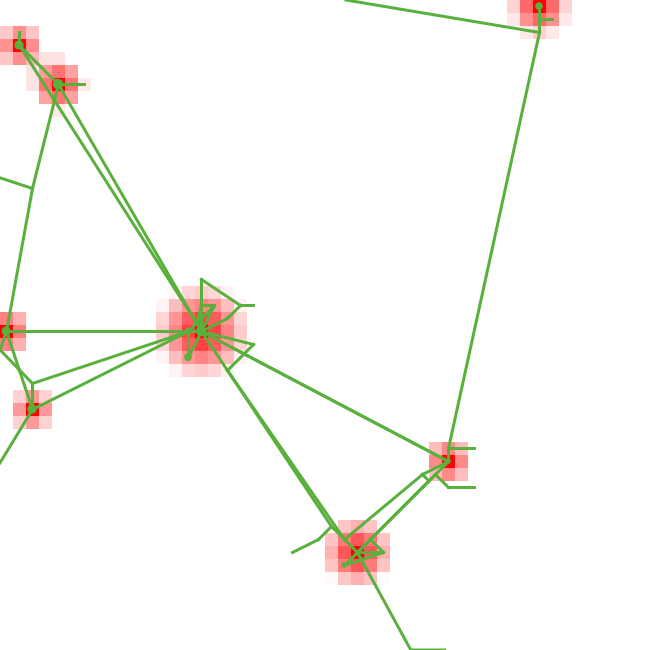
\includegraphics[width=0.32\textwidth]{figures/example_nwgrowth_tick2.png}}
\frame{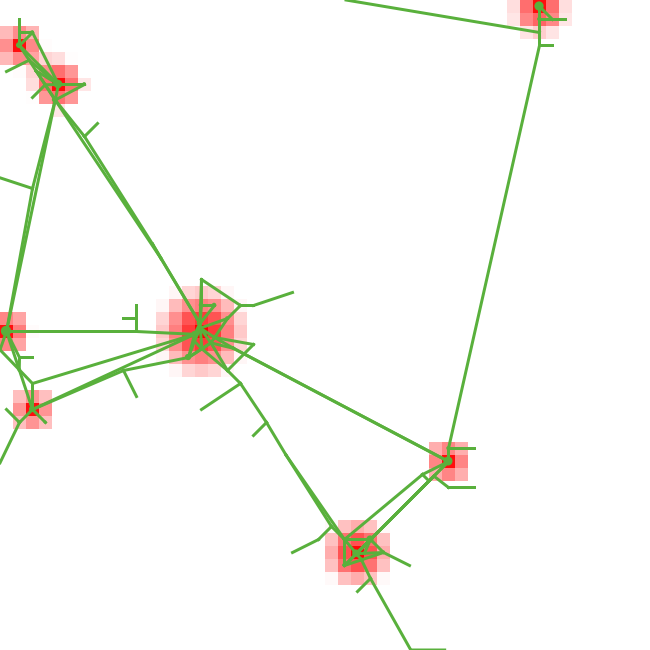
\includegraphics[width=0.32\textwidth]{figures/example_nwgrowth_tick10.png}}

}




\sframe{Biological network generation}{

Model studied by~\cite{tero2010rules} : exploration and reinforcement by a slime mould searching for ressources

\bigskip

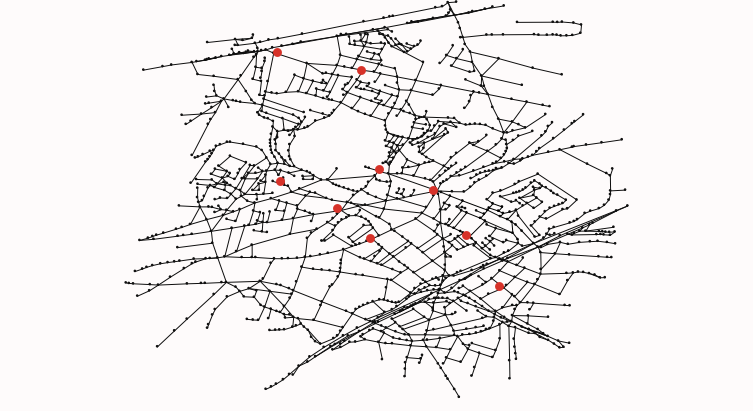
\includegraphics[width=0.32\textwidth]{figures/slimemould_tick1}
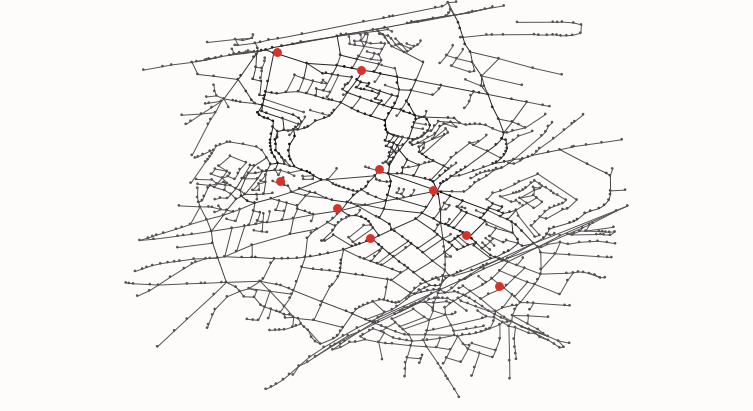
\includegraphics[width=0.32\textwidth]{figures/slimemould_tick10}
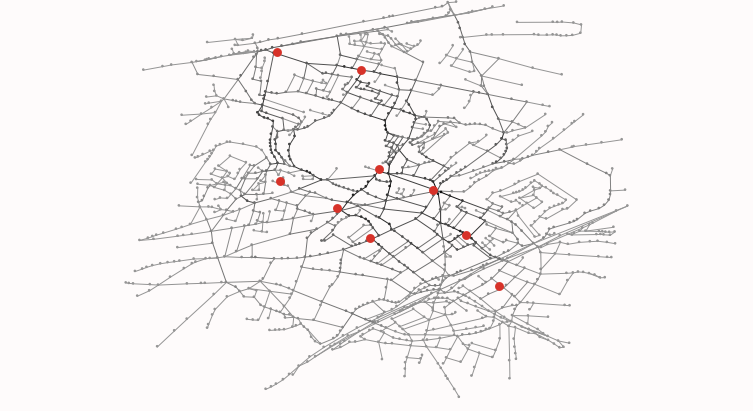
\includegraphics[width=0.32\textwidth]{figures/slimemould_tick20}\\
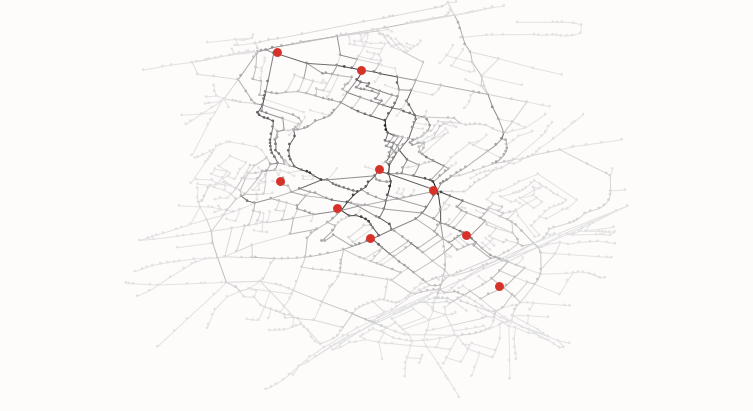
\includegraphics[width=0.32\textwidth]{figures/slimemould_tick50}
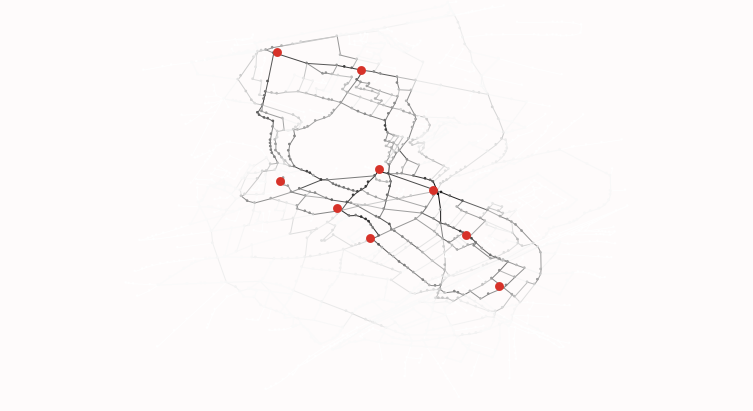
\includegraphics[width=0.32\textwidth]{figures/slimemould_tick101}
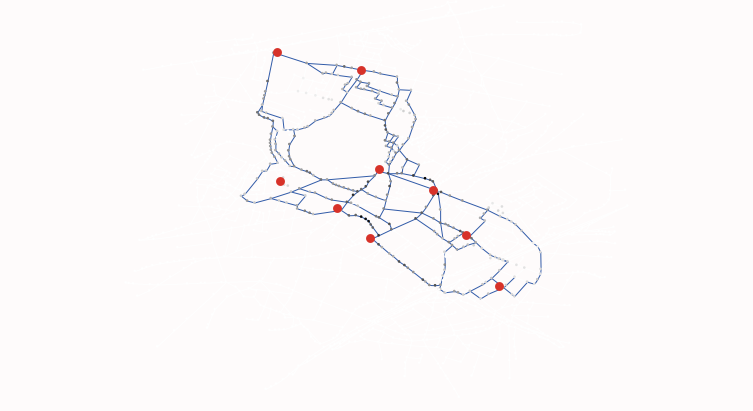
\includegraphics[width=0.32\textwidth]{figures/slimemould_reseauFinal}\\

\medskip

\footnotesize
\textit{Application to the design of optimal bus routes}

}




\sframe{Biological Network generation}{

Adding new links with biological heuristic:

\begin{enumerate}
	\item Create network of potential new links, with existing network and randomly sampled diagonal lattice
	\item Iterate for $k$ increasing ($k\in \{ 1,2,4 \}$ in practice) :
	\begin{itemize}
		\item Using population distribution, iterate $k\cdot n_b$ times the slime mould model to compute new link capacities
		\item Delete links with capacity under $\theta_d$
		\item Keep the largest connected component
	\end{itemize}
	\item Planarize and simplify final network
\end{enumerate}

\medskip

\centering

\frame{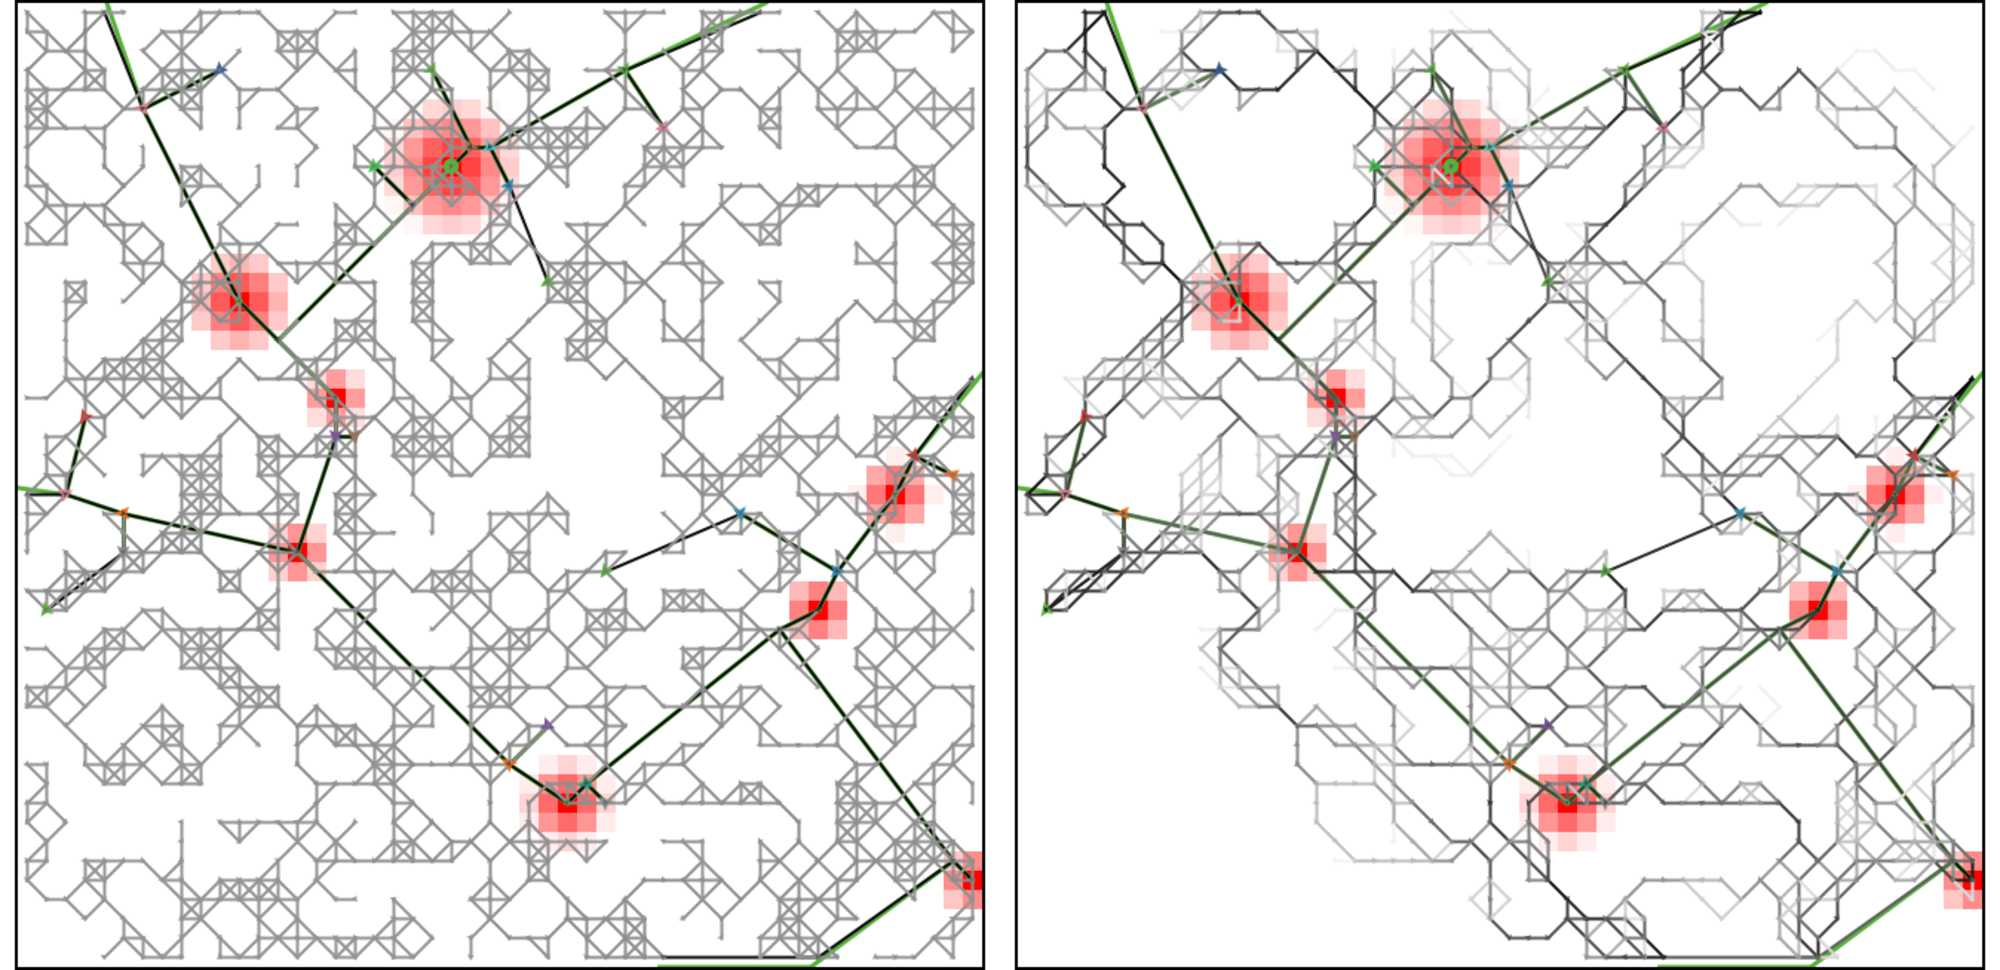
\includegraphics[width=0.6\textwidth]{figures/7-1-1-fig-networkgrowth-bioexample.jpg}}

\footnotesize

\textit{Intermediate stage for biological network generation}

}



\sframe{Generated Urban Shapes: Network}{


\centering

\frame{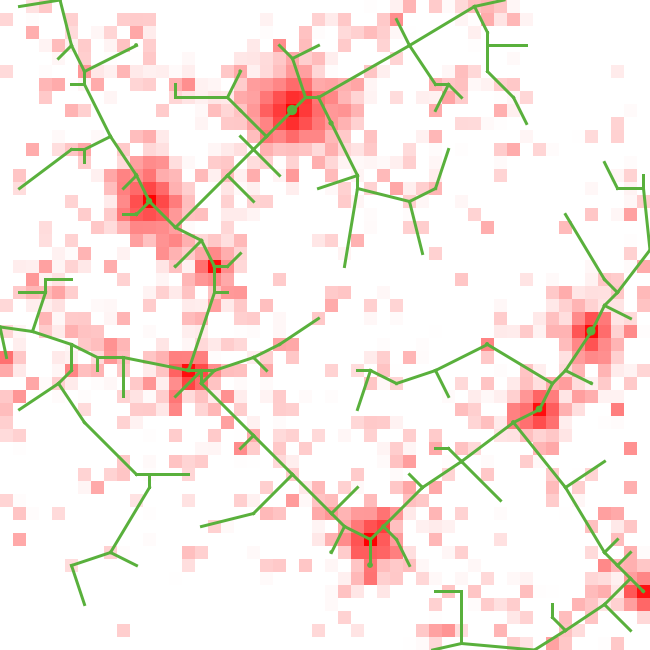
\includegraphics[width=0.28\textwidth]{figures/coevol_example_nw-connection}}\hspace{0.1cm}
\frame{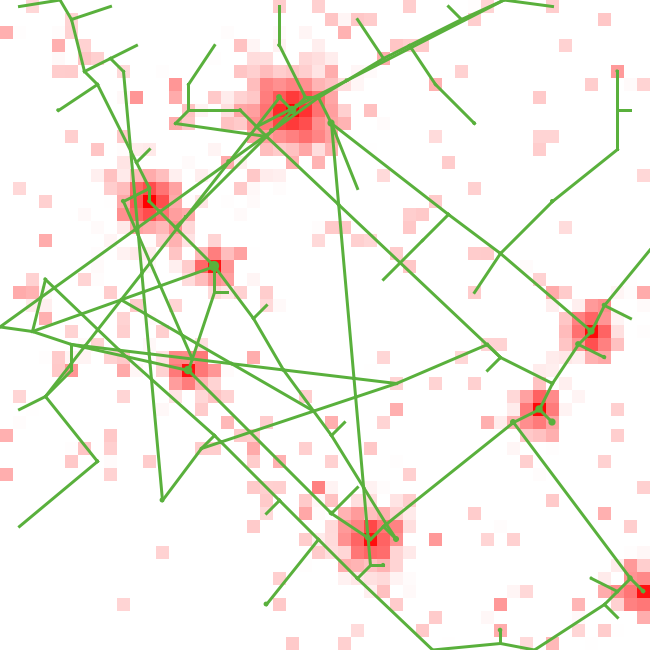
\includegraphics[width=0.28\textwidth]{figures/coevol_example_nw-random}}\hspace{0.1cm}
\frame{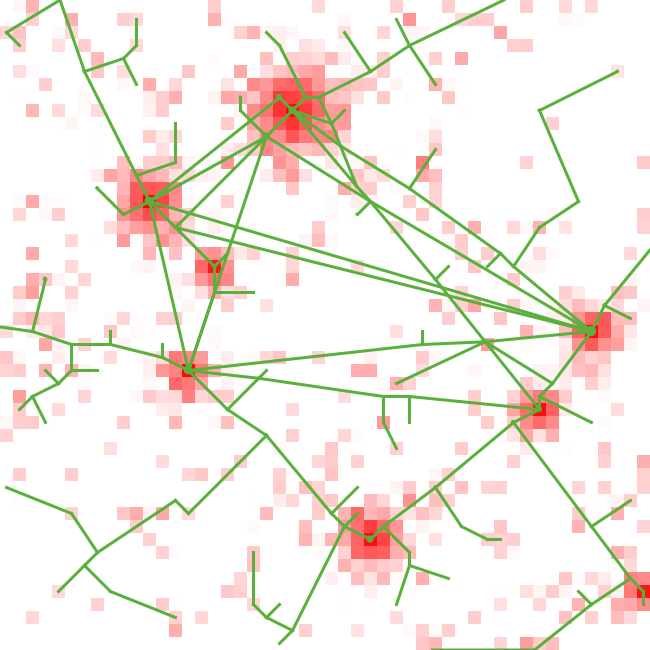
\includegraphics[width=0.28\textwidth]{figures/coevol_example_nw-gravity}}\\\vspace{0.1cm}
\frame{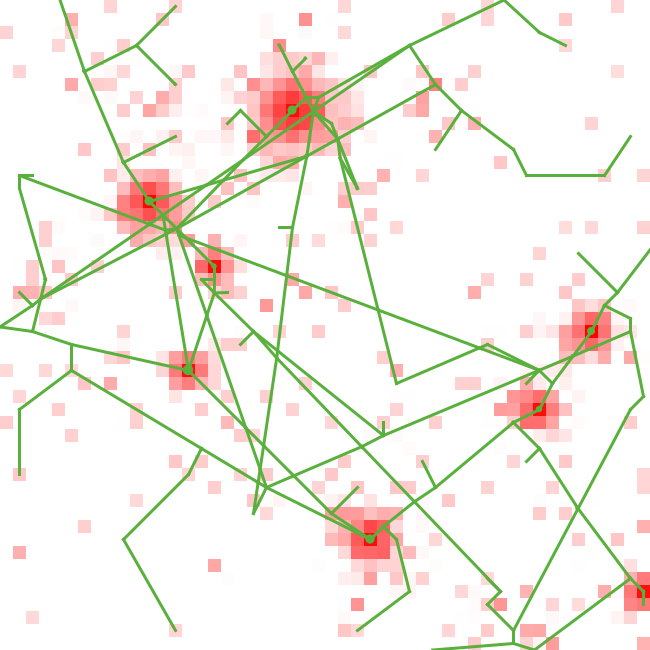
\includegraphics[width=0.28\textwidth]{figures/coevol_example_nw-rndbrkdwn}}\hspace{0.1cm}
\frame{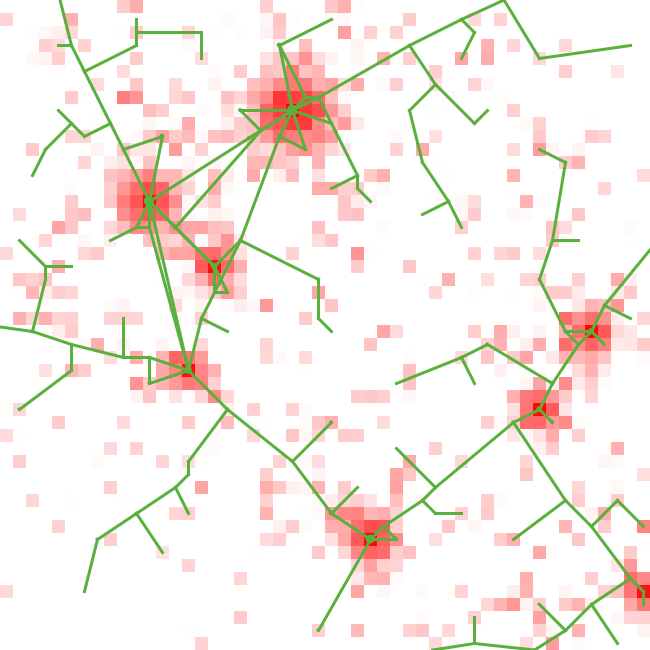
\includegraphics[width=0.28\textwidth]{figures/coevol_example_nw-cost}}\hspace{0.1cm}
\frame{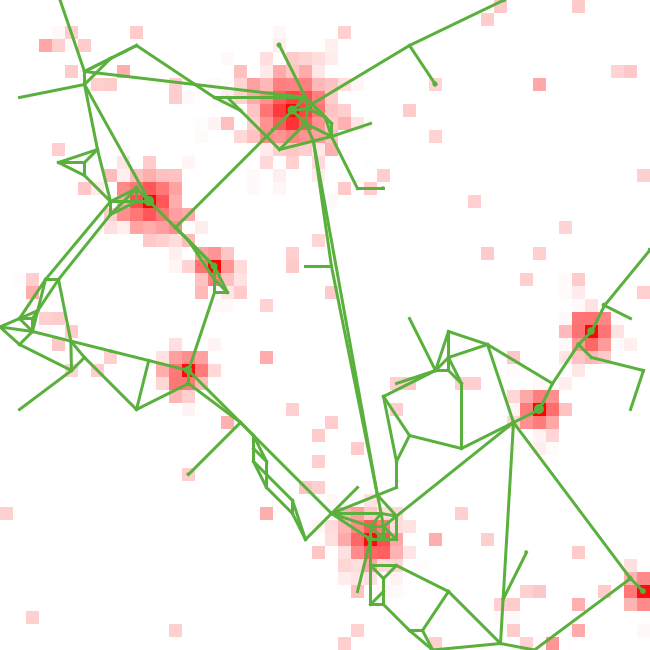
\includegraphics[width=0.28\textwidth]{figures/coevol_example_nw-bio}}

\footnotesize\textit{In order: connection; random; deterministic breakdown; random breakdown; cost-driven; biological.}

}




\sframe{Synthetic systems of cities}{


\textit{At the macroscopic scale: synthetic systems of cities}


\begin{itemize}
	\item Evolutive urban theory: systems of cities follow general stylized facts \cite{pumain2018evolutionary}
	\item Rank-size law \cite{pumain2006evolutionary}
	\item Central place theory
\end{itemize}


}

\sframe{Cities and networks}{

% simpopnet generator

\textit{Synthetic system of cities and network for the SimpopNet model} \cite{raimbault2018unveiling}

\medskip

\begin{center}
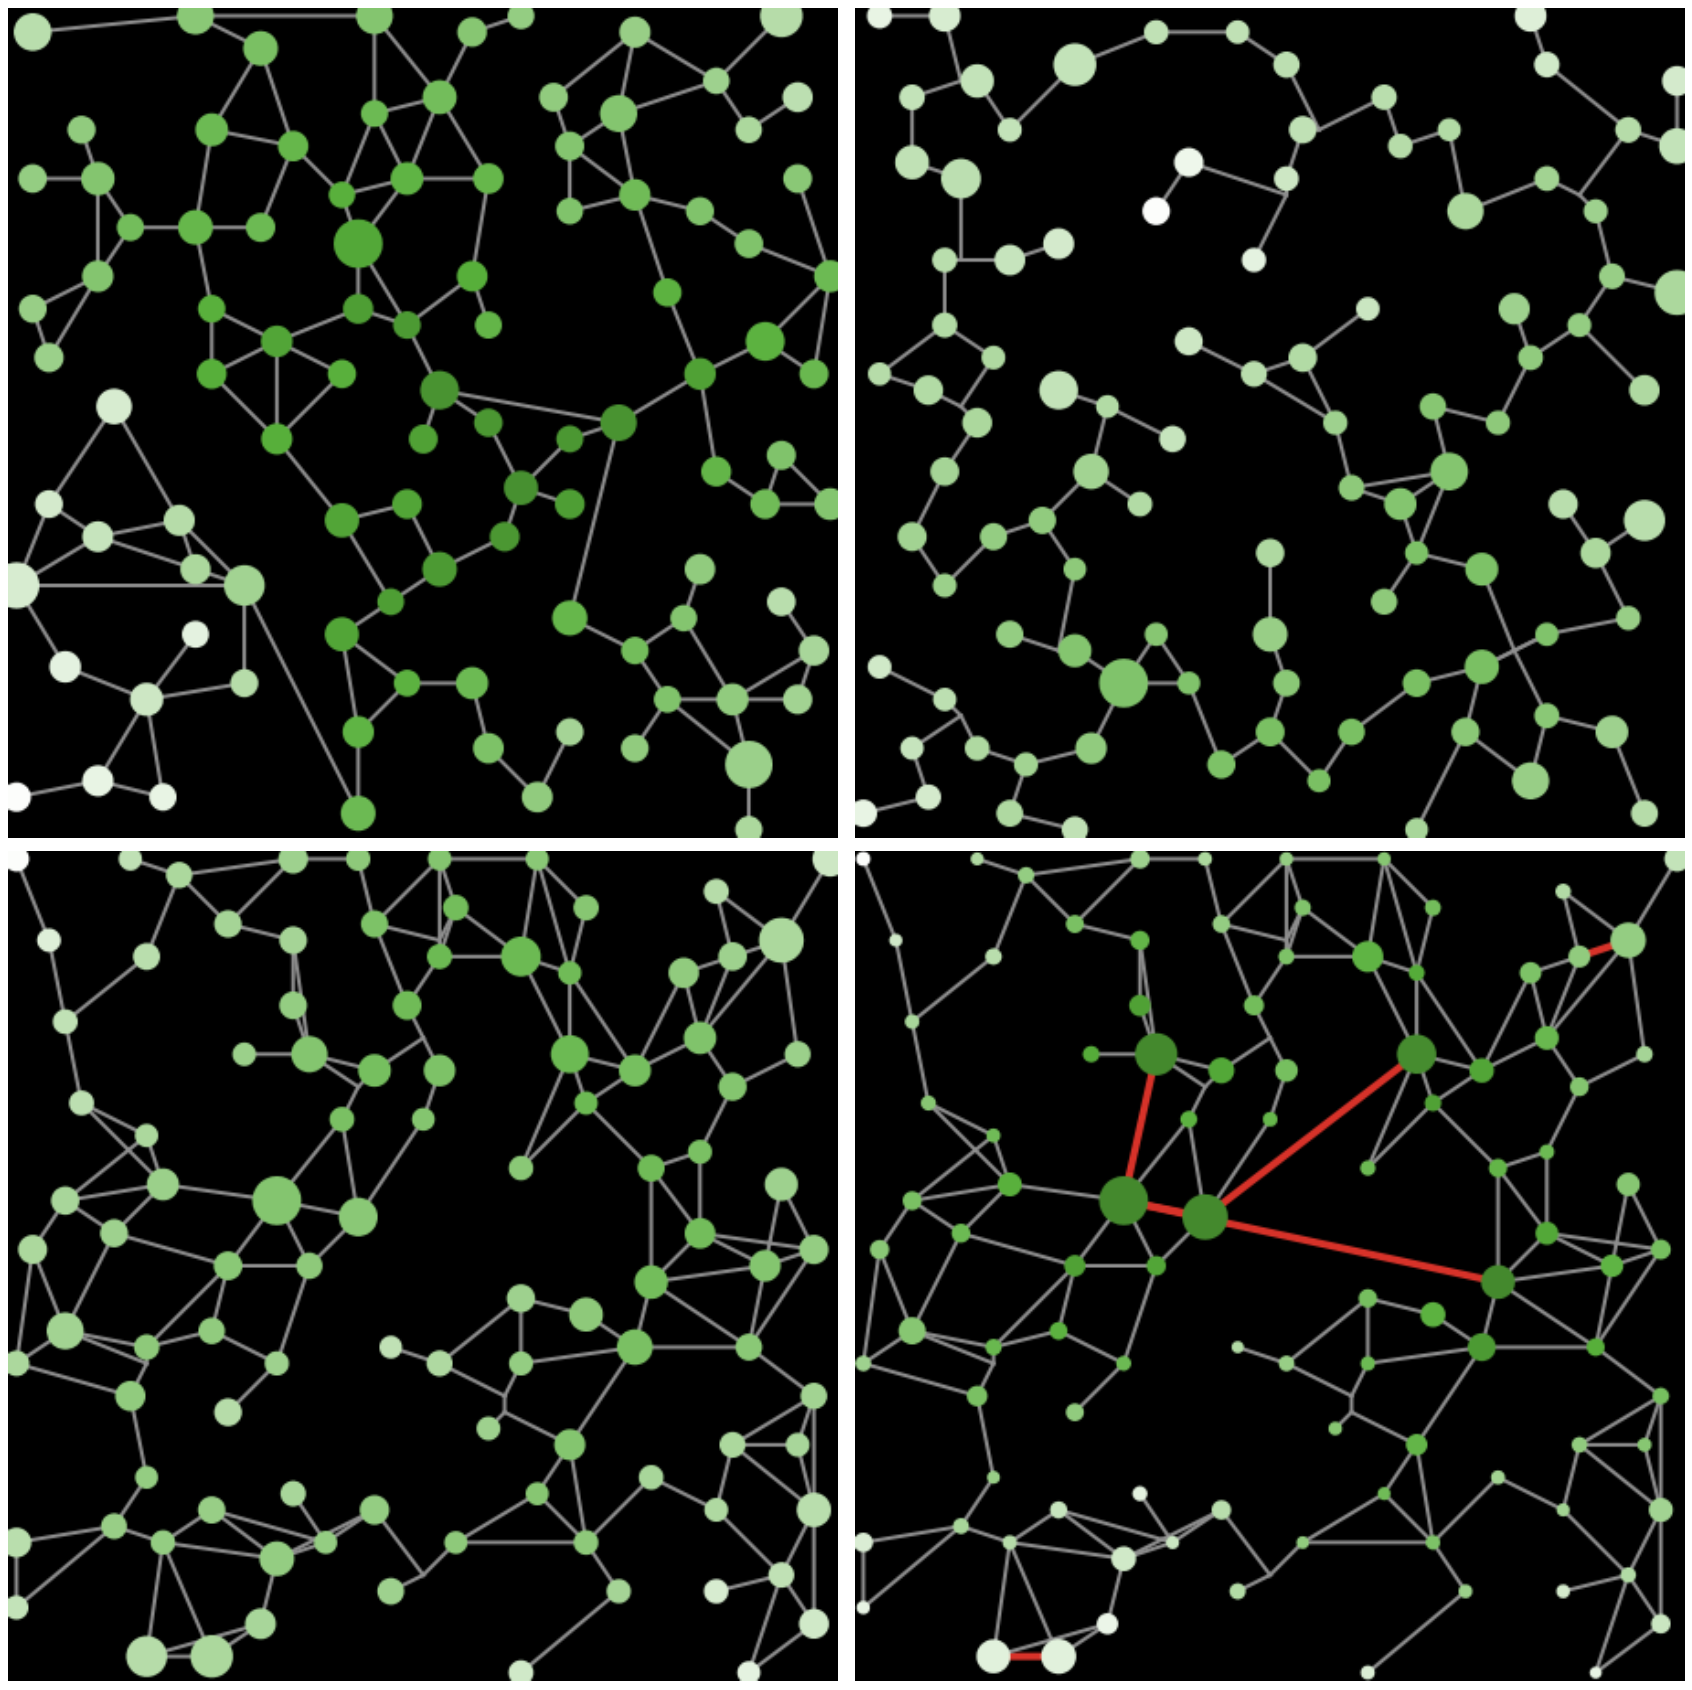
\includegraphics[height=0.75\textheight]{figures/simpopnet_Fig1.png}
\end{center}


}

\sframe{Cities and networks}{

% ex from cities nw paper

\textit{Cities-network co-evolution model explored on synthetic systems of cities} \cite{raimbault2019modeling}

\medskip

\begin{center}
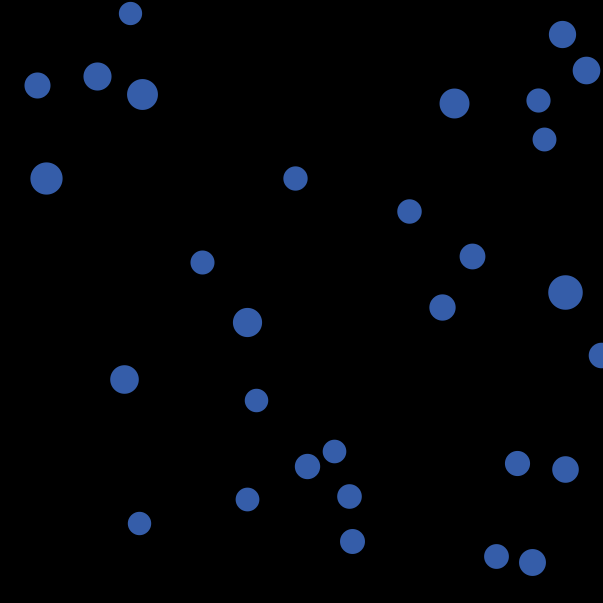
\includegraphics[height=0.47\textheight]{figures/macrocoevol_example_virtual_0_t0.png}\hspace{0.2cm}
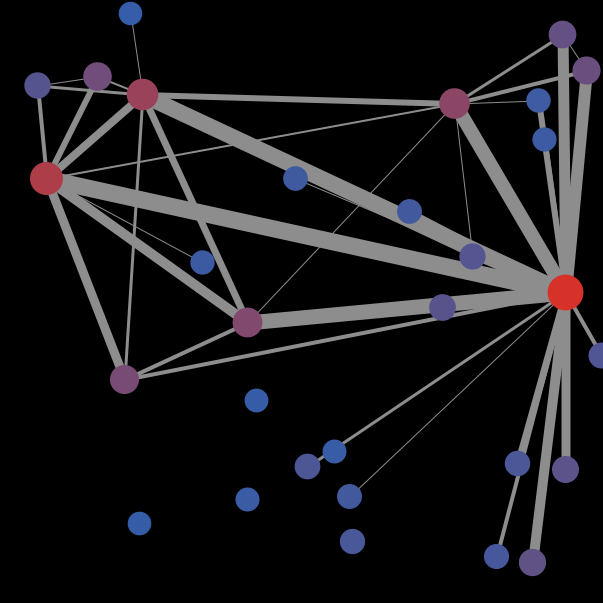
\includegraphics[height=0.47\textheight]{figures/macrocoevol_example_virtual_0_tf.png}
\end{center}


}




\subsection{Perturbation of real data}



\sframe{Real data perturbation}{


\textit{currently being implemented}

\medskip

$\rightarrow$ \textit{How does noise in real data impacts the result ?}


\medskip

\begin{itemize}
	\item Impact of missing elements
	\item Impact of imprecise coordinates or topology
	\item Optimal matching between spatial datasets
\end{itemize}


\bigskip

$\rightarrow$ \textit{How does perturbation of real data allows to explore scenario}

\medskip

\textbf{Examples:}

\begin{itemize}
   \item simulating urban projects by modifying population of areas with a given spatial correlation structure %Forcity example
	\item simulating network disruptions or new transportation lines
\end{itemize}


}



\subsection{Indicators}



\section{Spatial indicators for model outputs}


\sframe{Spatial statistics}{

\textit{In the spatial approach, spatial model indicators are also important: what kind of spatial structure does the model produce ?}

\bigskip 
 
 \begin{itemize}
 	\item previous form indicators at different scales, applied on any spatialized variable or event: quantify level of aggregation, hierarchy, clustering
 	\item spatial statistics indicators and methods
 	\item more complicated approaches: fractals and multifractals, spatial datamining
 \end{itemize}

}




\subsection{Integration into OpenMOLE}


\sframe{Integration into OpenMOLE}{

}





\section{Applications}


\subsection{Calibration of generators}


\sframe{Large scales: real urban configurations}{

\textit{Sampled districts from OpenStreetMap}

%\medskip

\begin{center}
	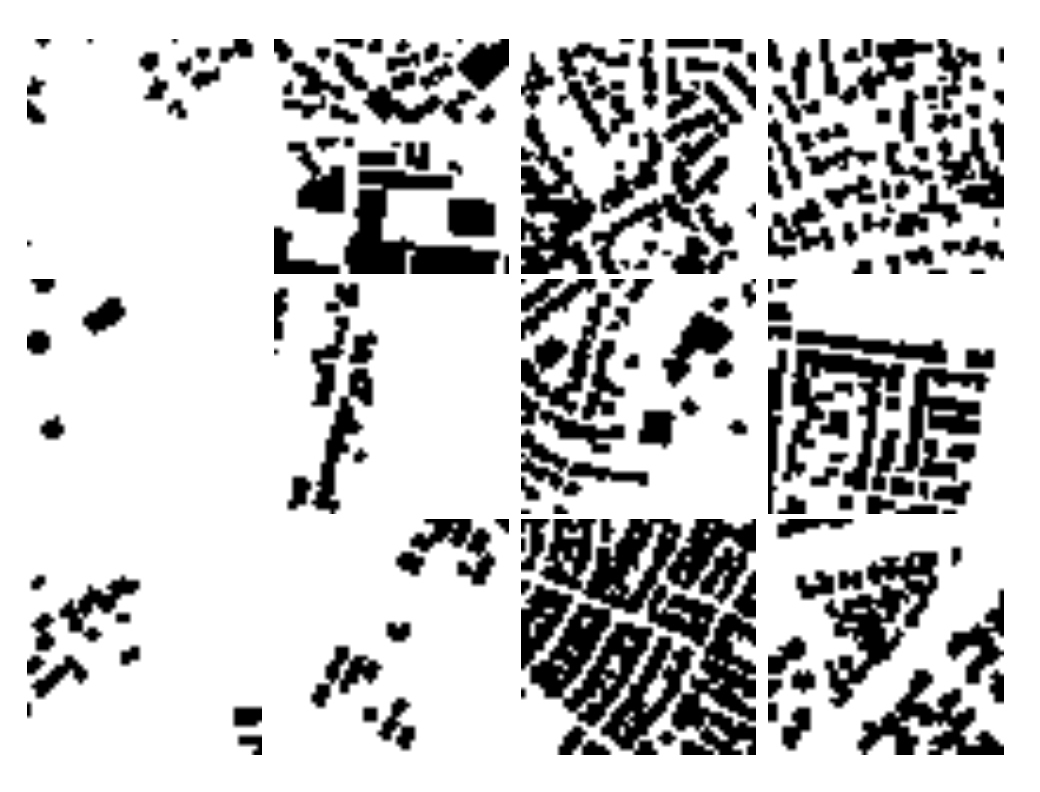
\includegraphics[height=0.85\textheight]{figures/spatialsens_exampleosm.png}
\end{center}

}


\sframe{Classification of urban forms}{

\begin{center}
   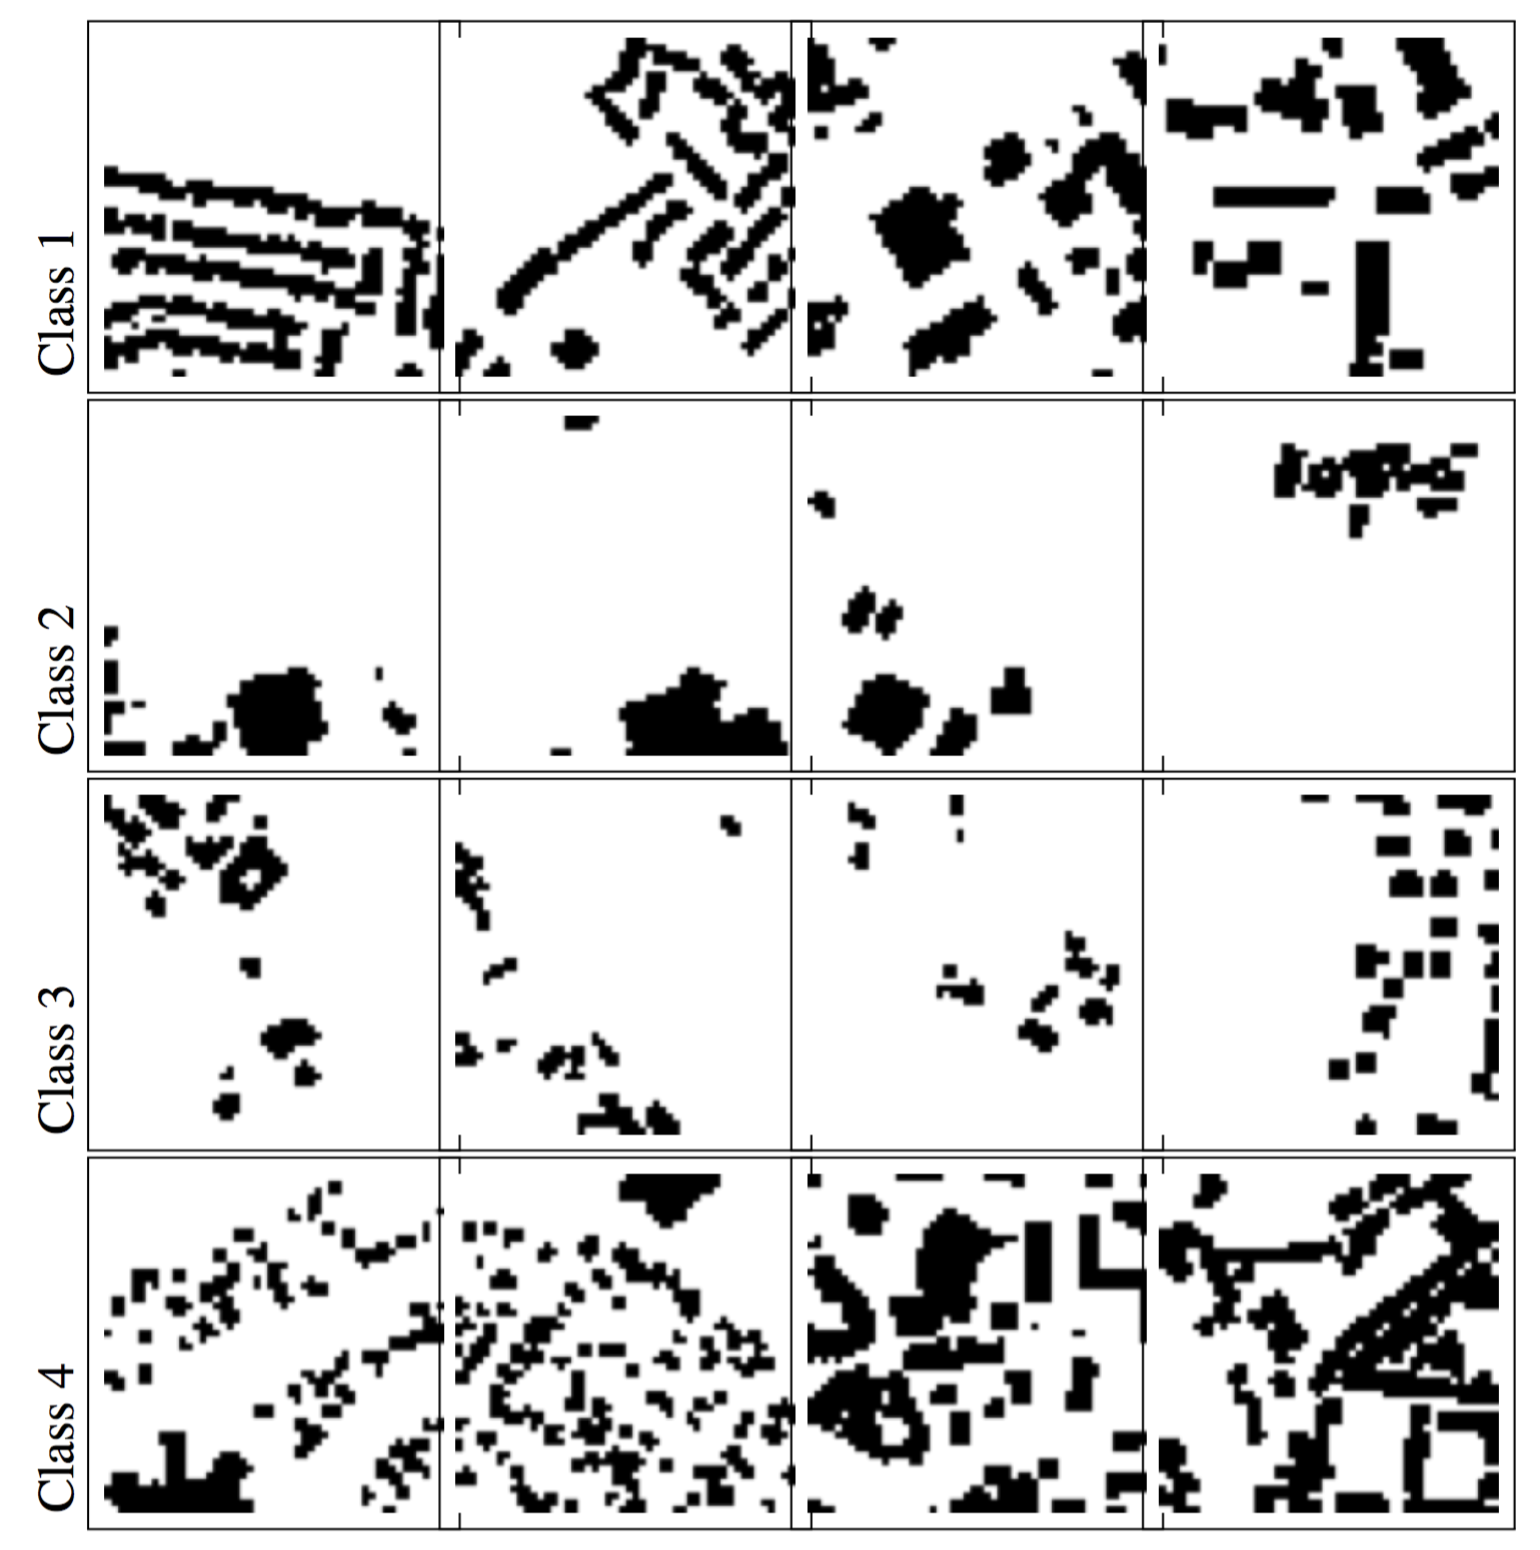
\includegraphics[height=0.9\textheight]{figures/spatialsens_osm_classification.png}
\end{center}

}


\sframe{Calibrated forms}{

\centering

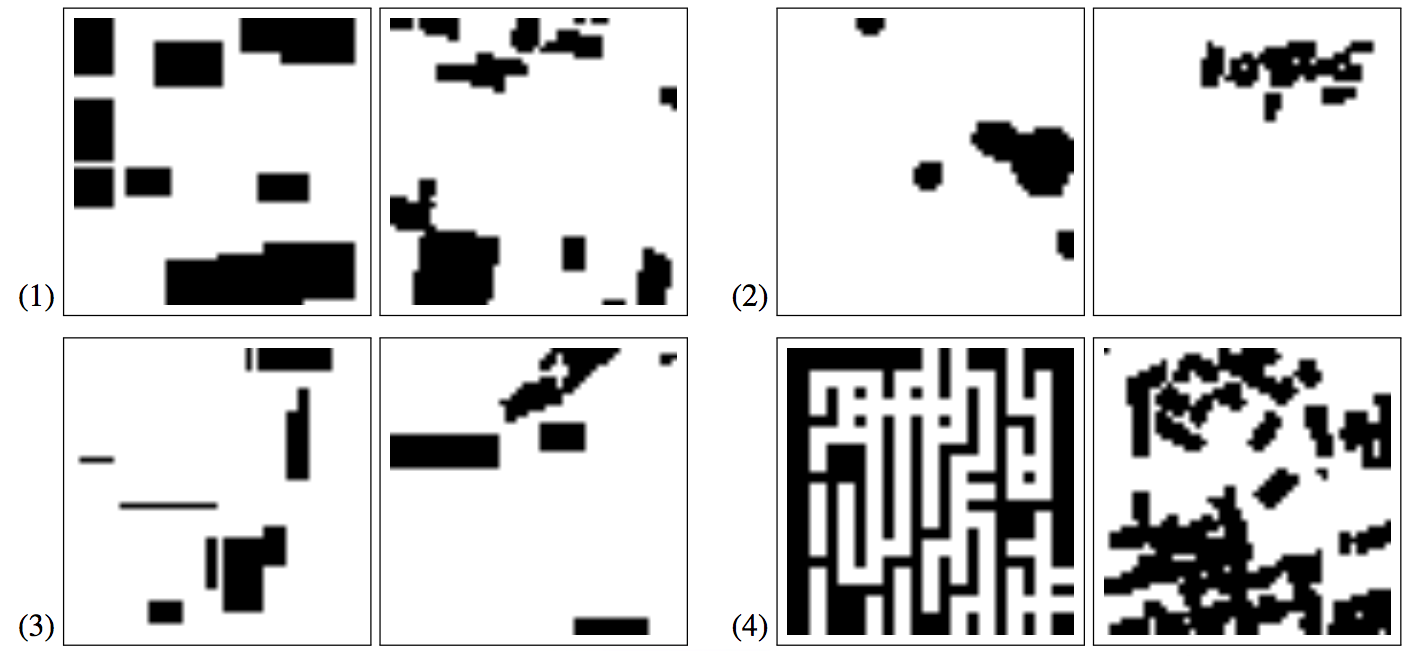
\includegraphics[width=\textwidth]{figures/spatialsens_calib.png}

}


\sframe{Point cloud}{

\begin{center}
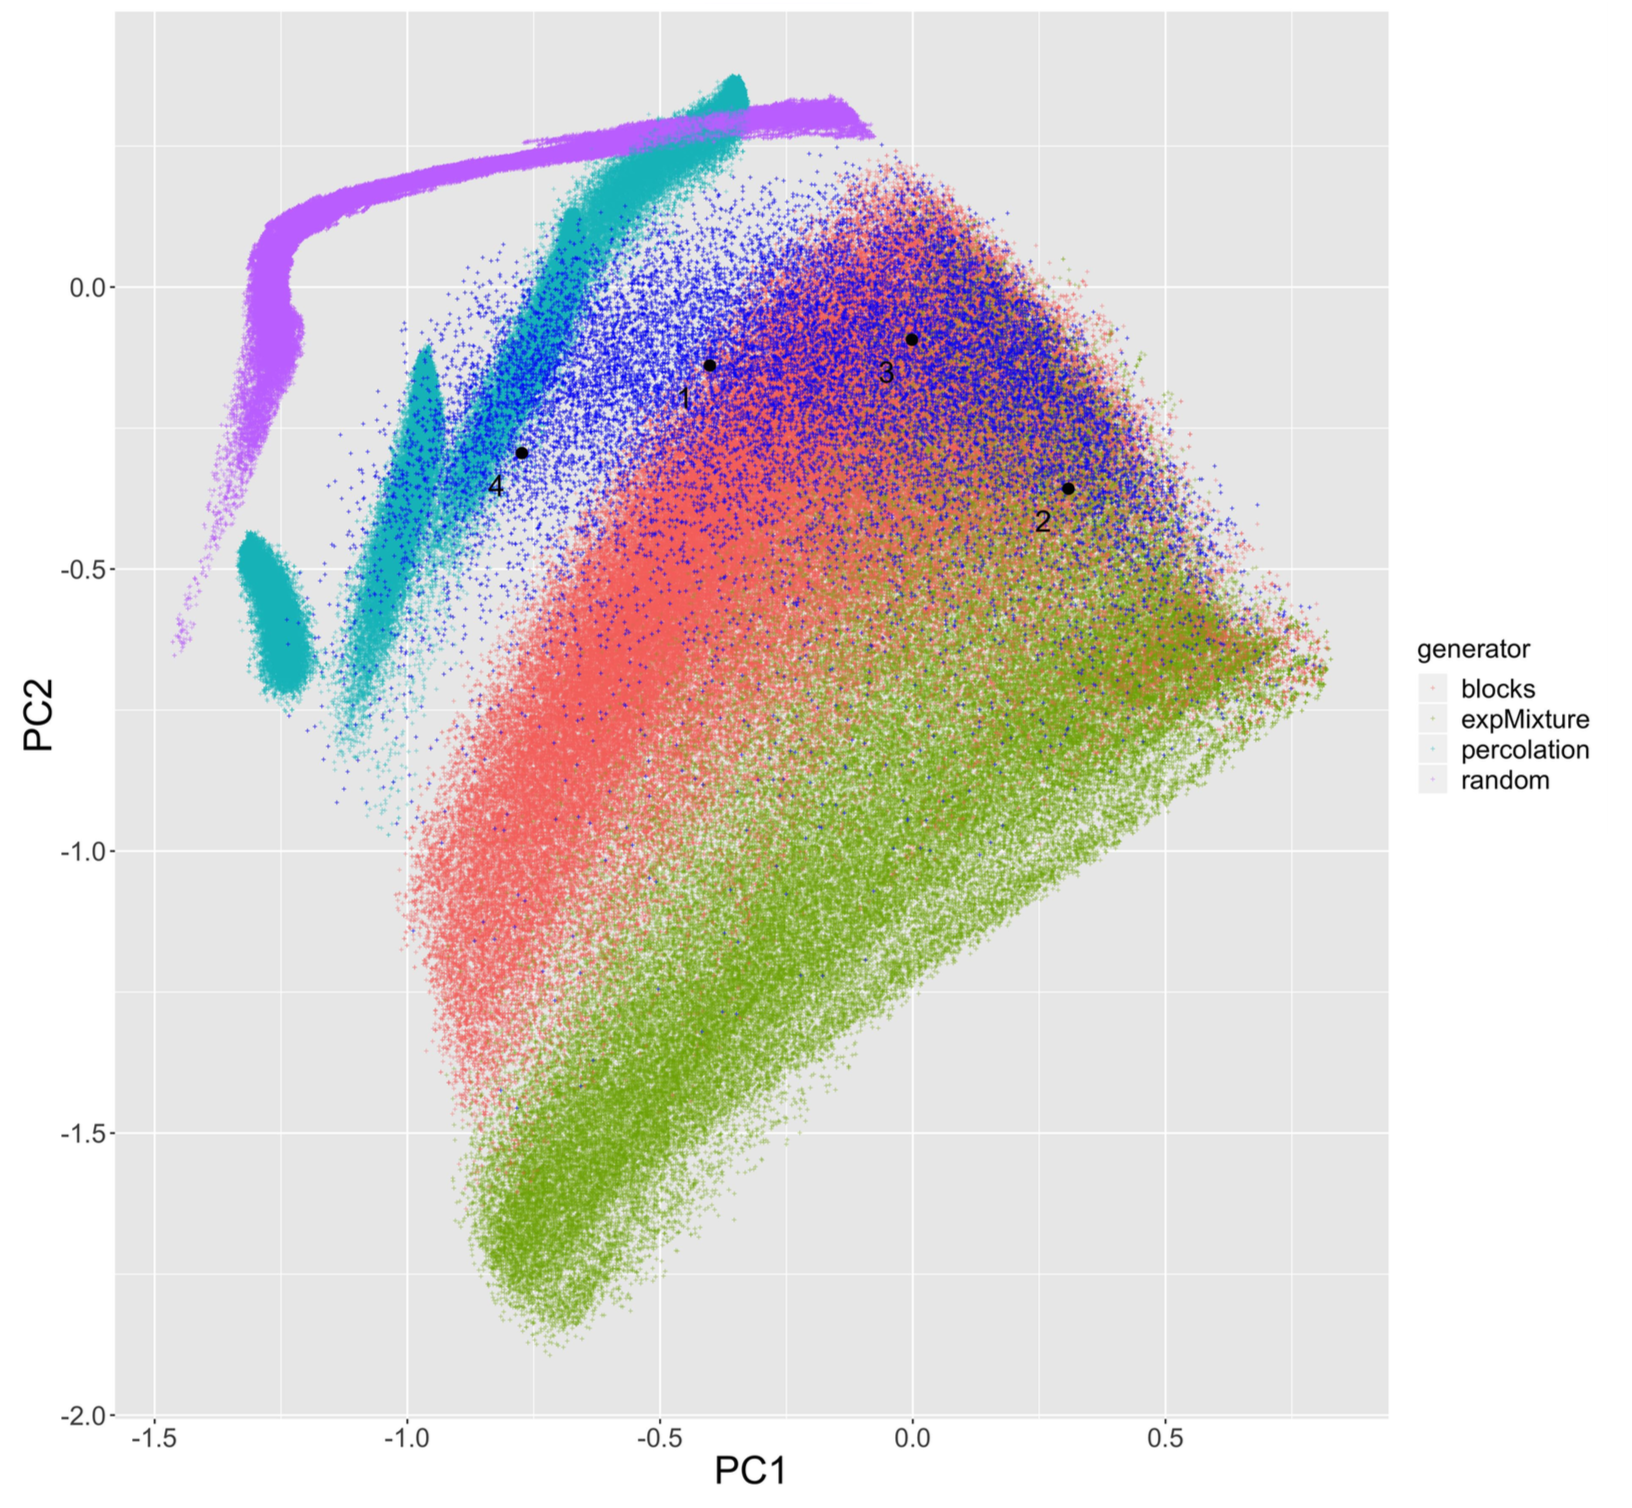
\includegraphics[height=0.9\textheight]{figures/spatialsens_points.png}
\end{center}

}


\sframe{Calibration}{

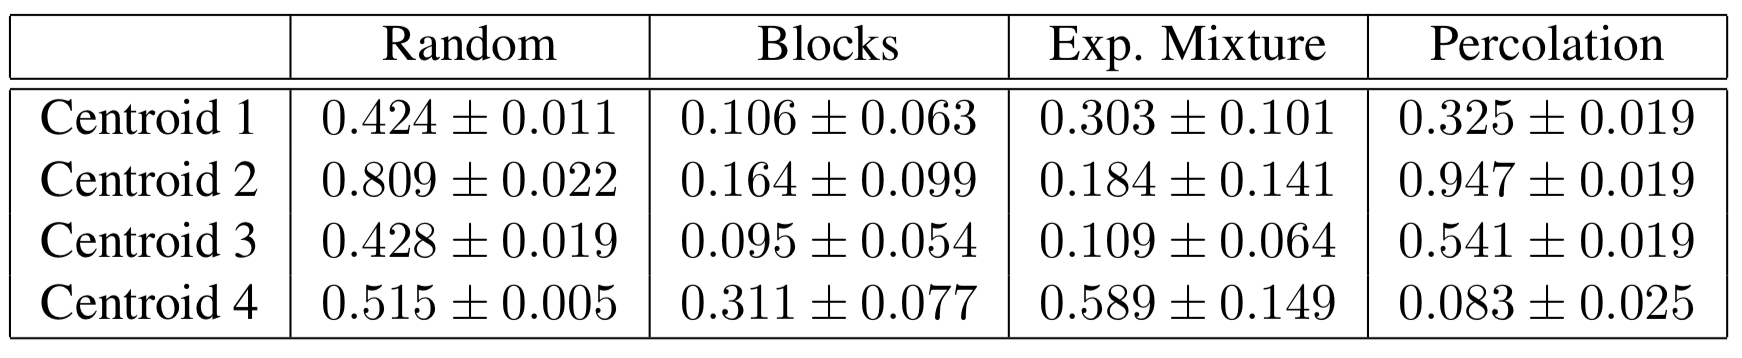
\includegraphics[width=\textwidth]{figures/spatialsens_distanceclasses.png}

\medskip

\textit{Why not use calibration heuristics? Open question of fitting a point cloud; issue of projecting in a reduced dimension space}

}


\sframe{Implementation in OpenMOLE}{

% spatialsmapling syntax 

\begin{center}
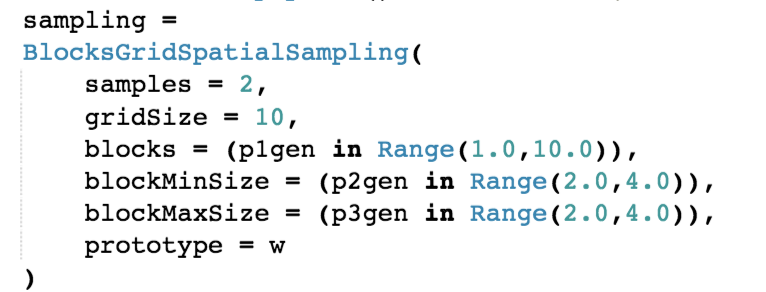
\includegraphics[width=0.8\textwidth]{figures/blocksampling.png}
\end{center}

\medskip

\justify

$\rightarrow$ other generators have their own primitives\\(\texttt{ExpMixtureThresholdSpatialSampling},\\ \texttt{PercolationGridSpatialSampling}) and arguments (\textbf{see the documentation})

}




\sframe{Population grids: empirical Data for Calibration}{


\begin{columns}
\column{0.6\textwidth}
\centering
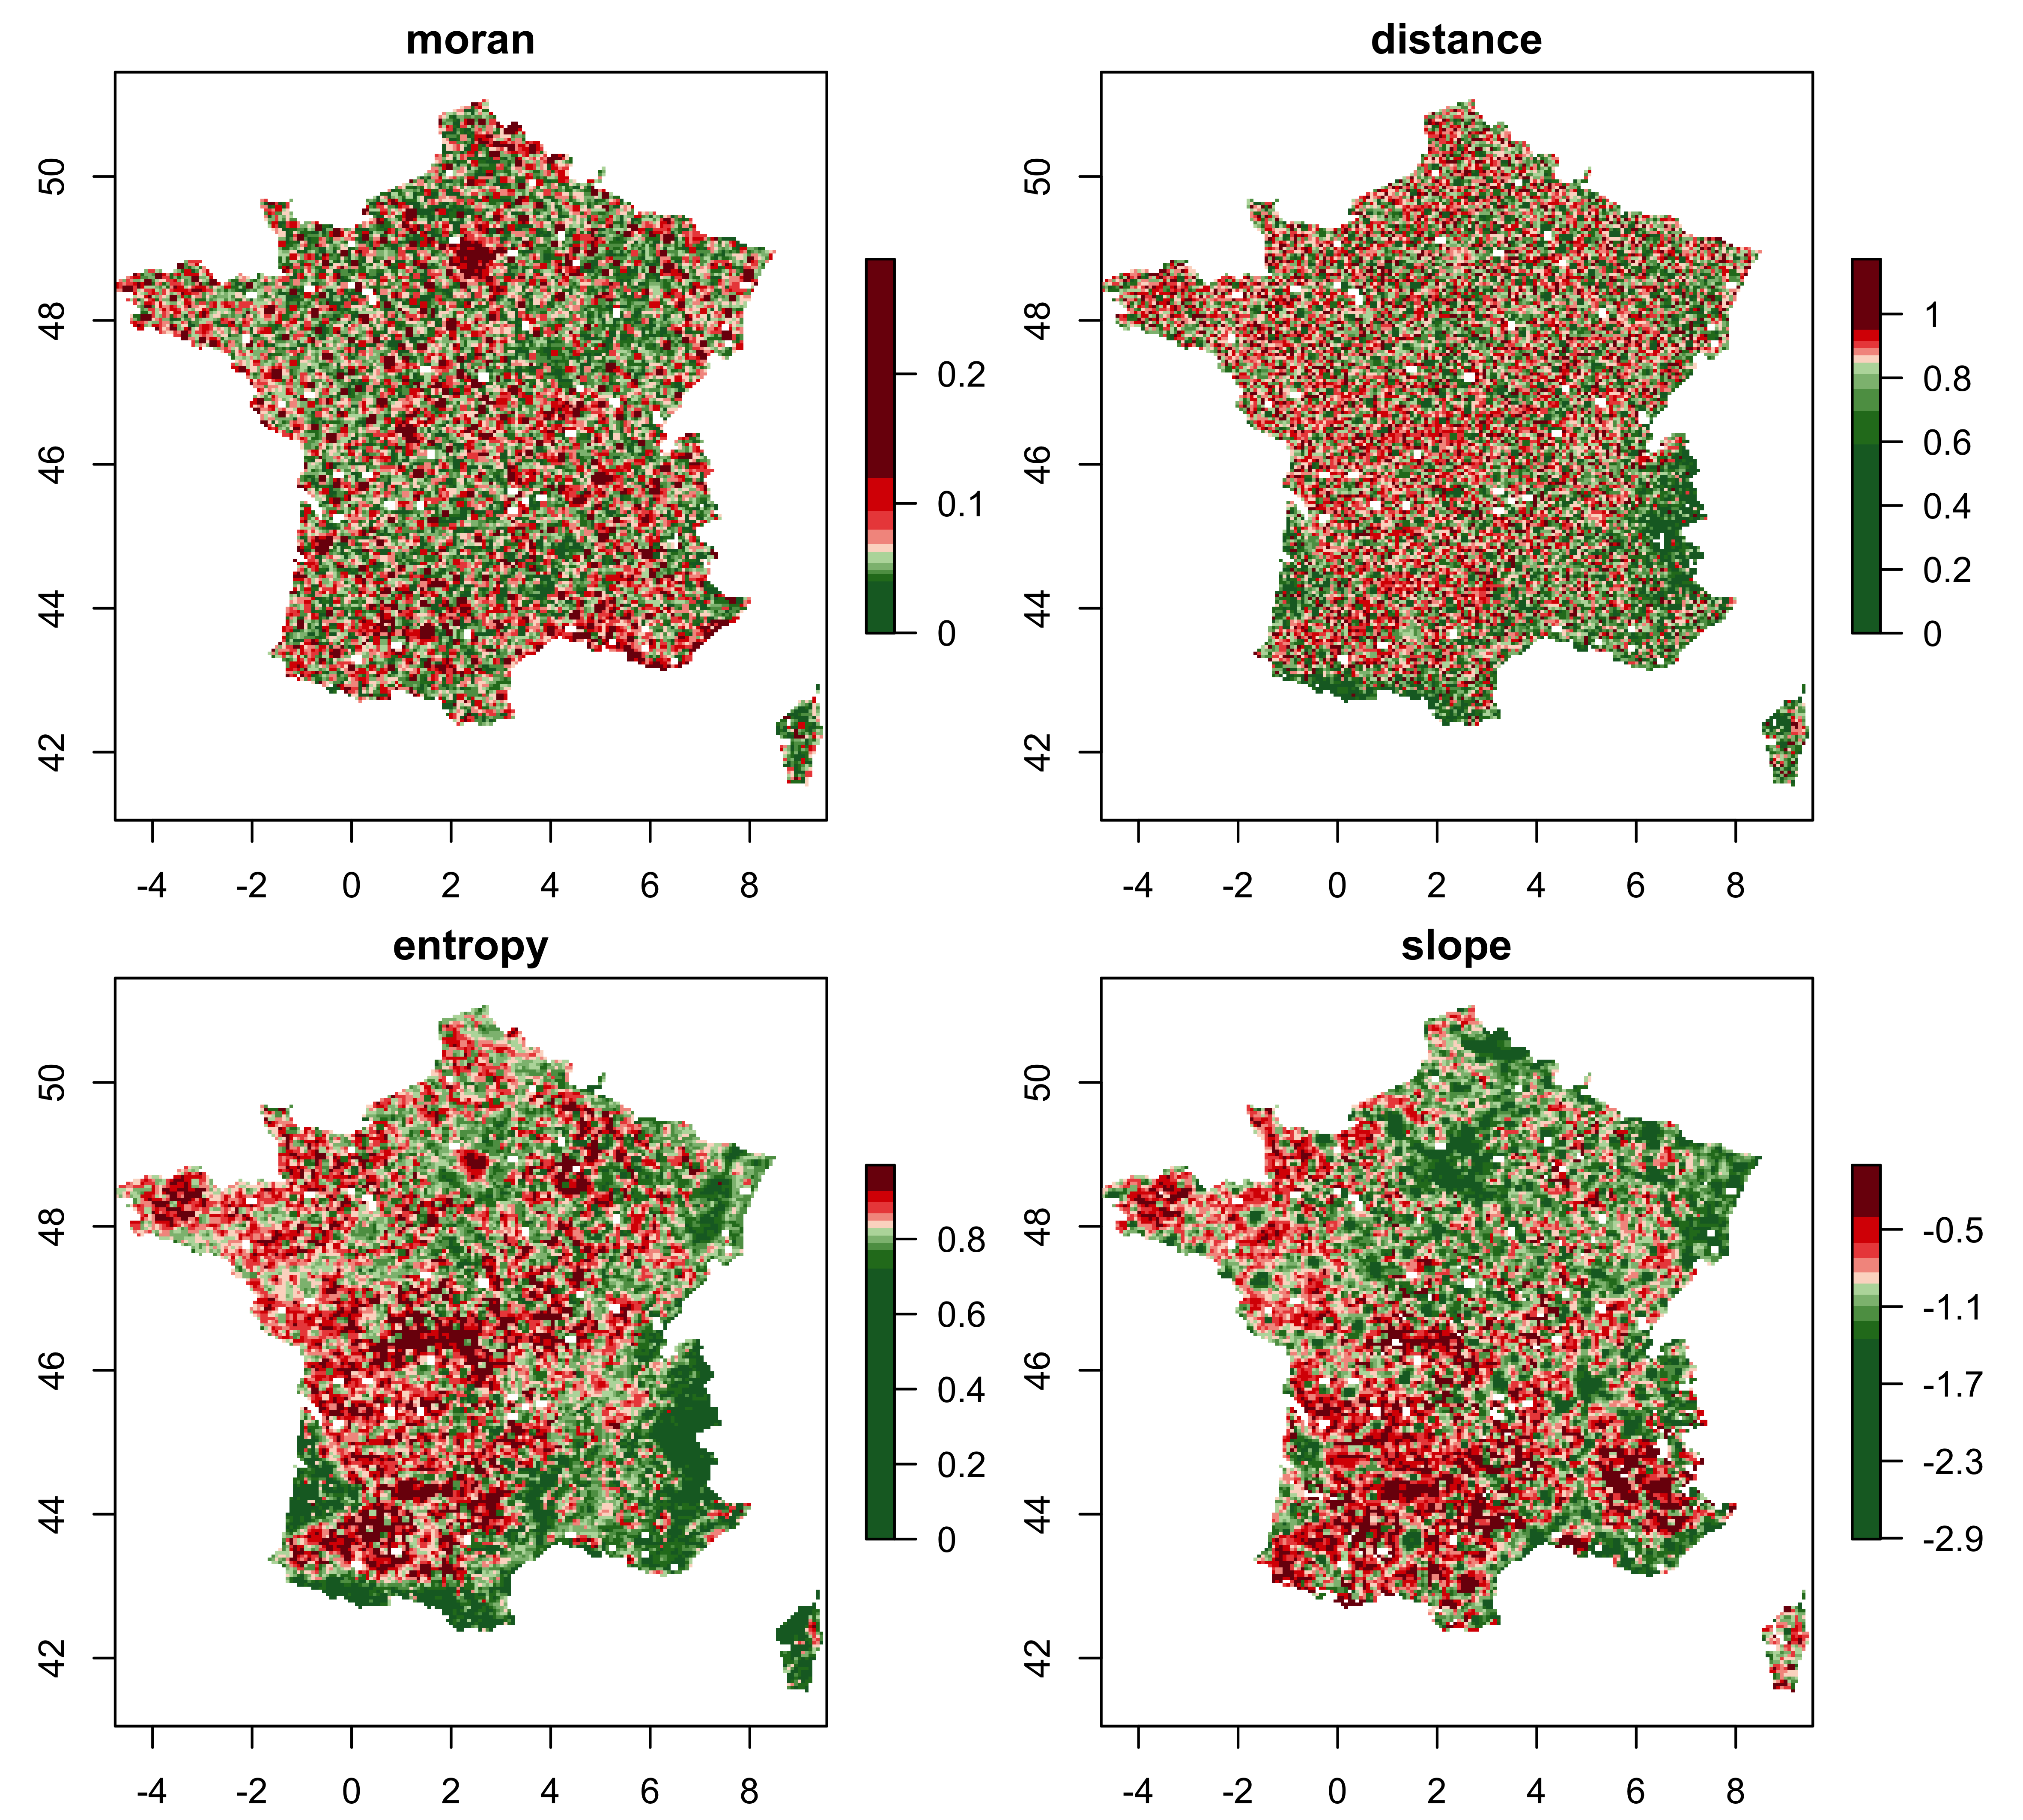
\includegraphics[width=\textwidth]{figures/density_indics_morpho_discrquantiles}
\column{0.3\textwidth}
\centering
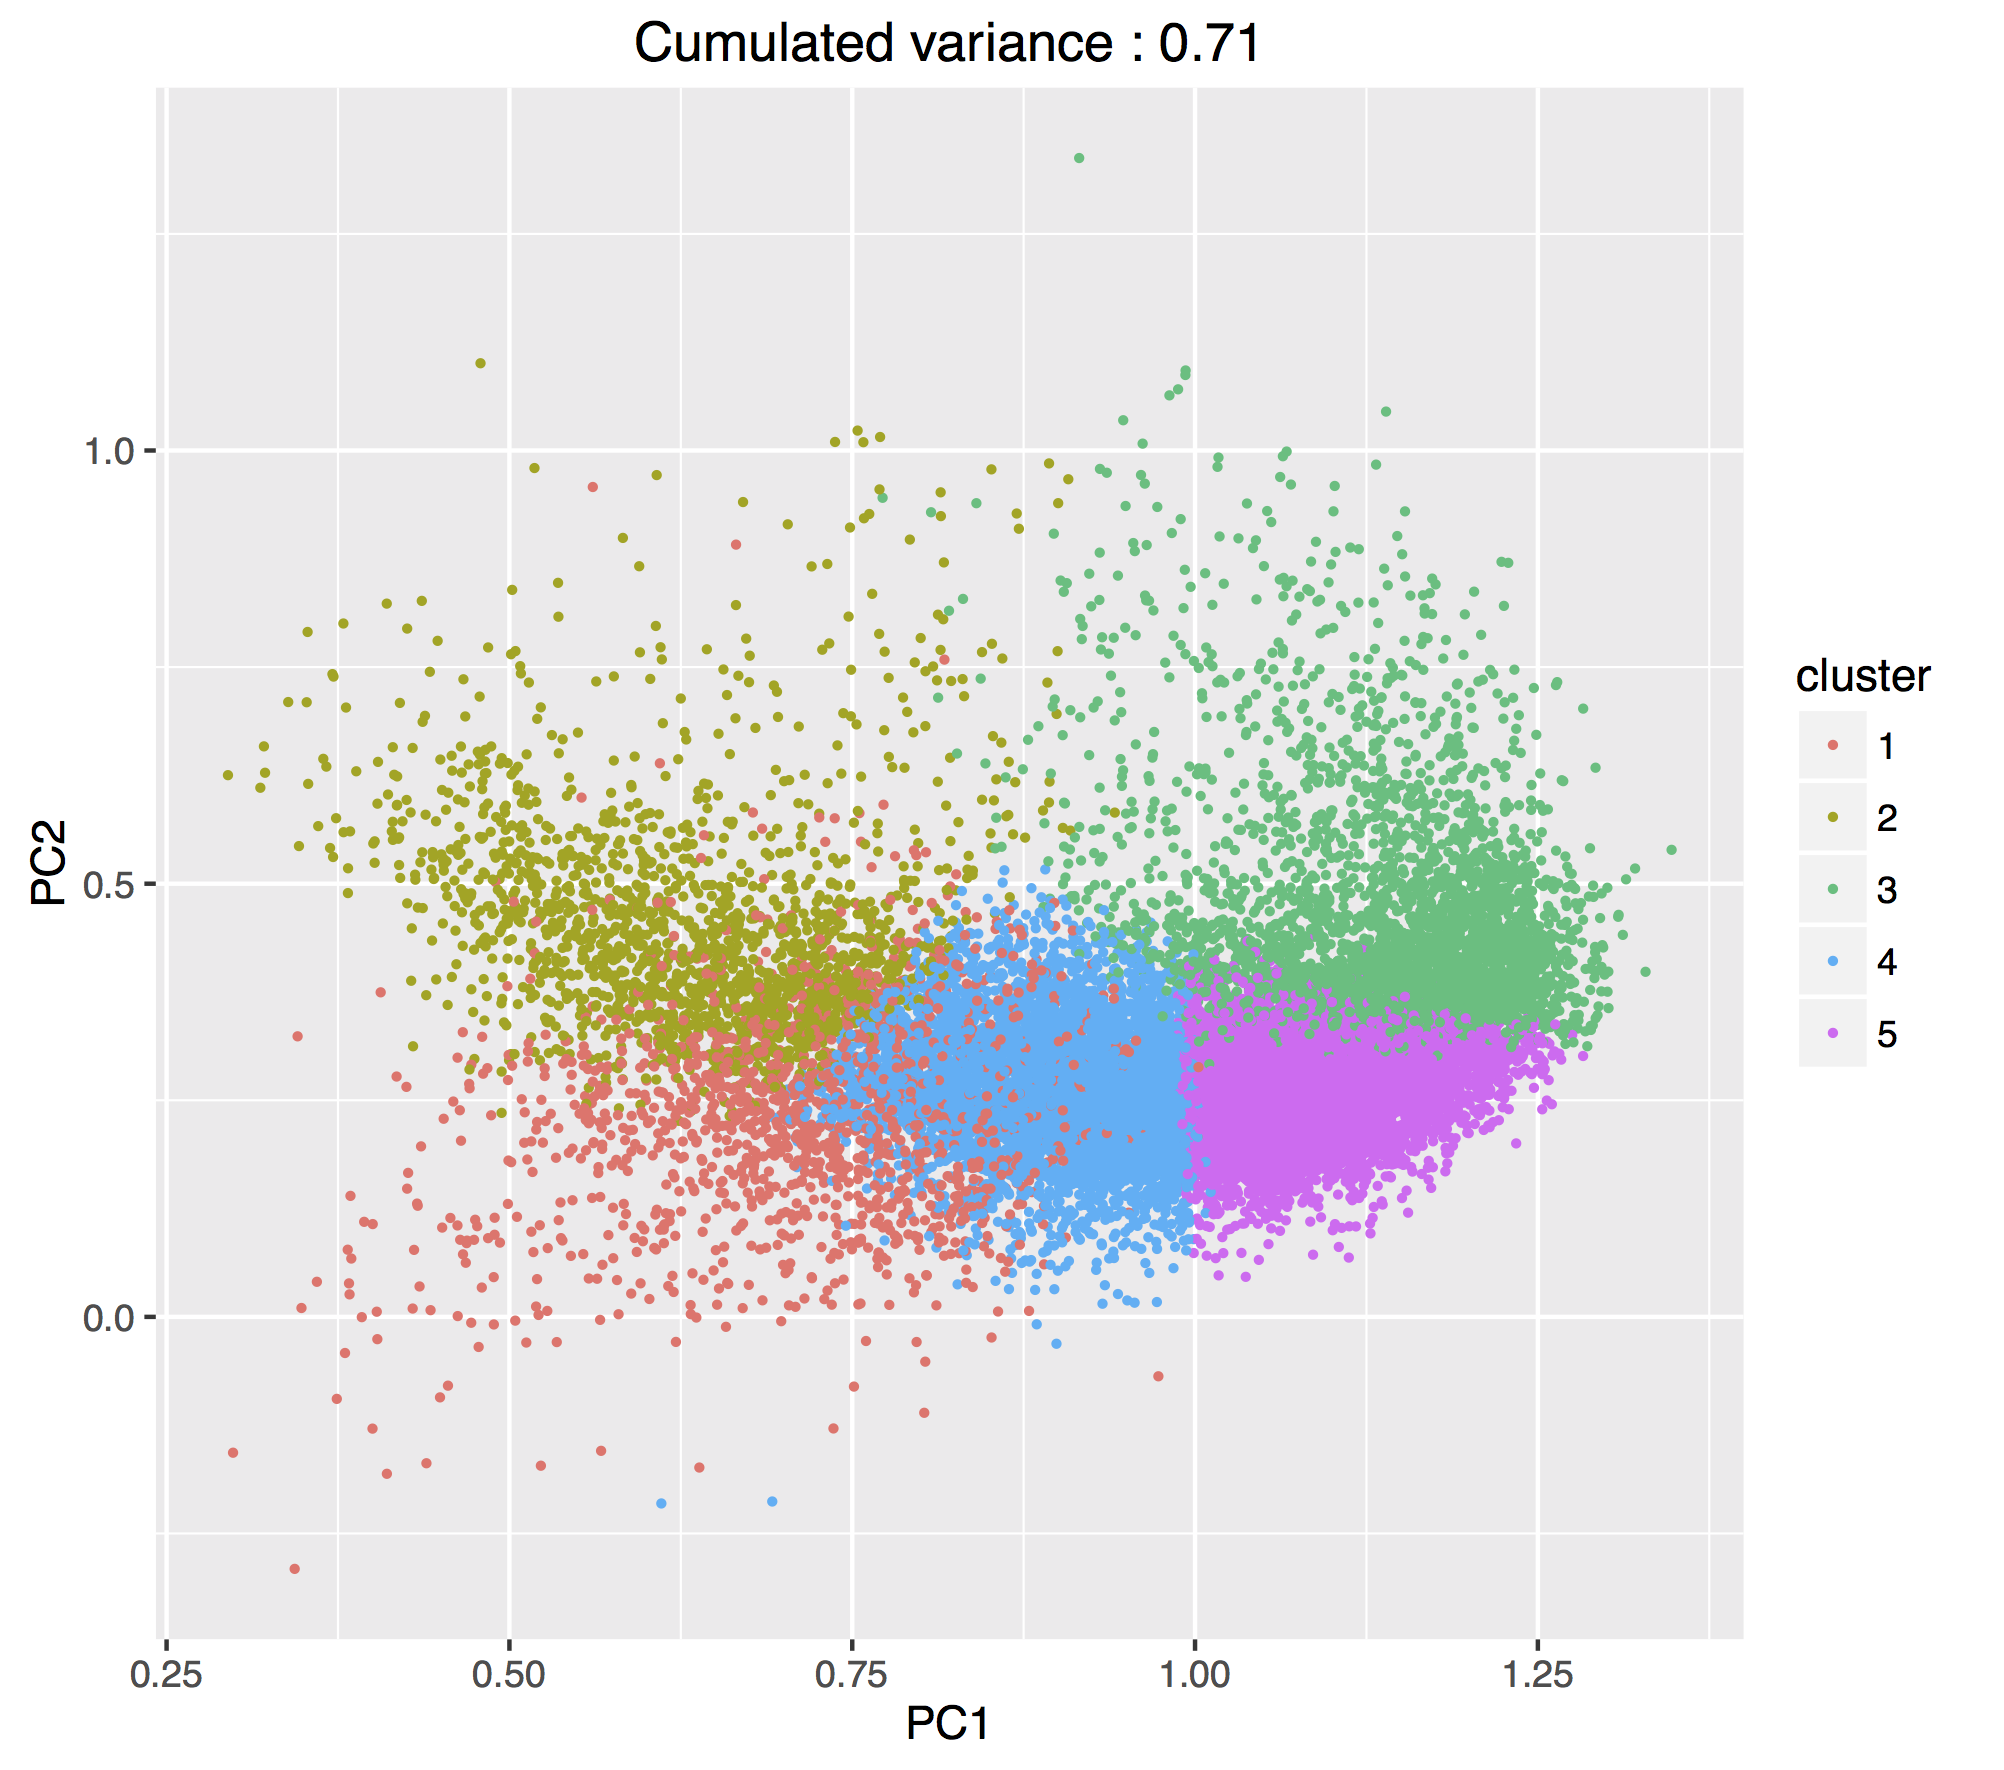
\includegraphics[width=\textwidth]{figures/density_cluster_pca_k5_morpho}\\
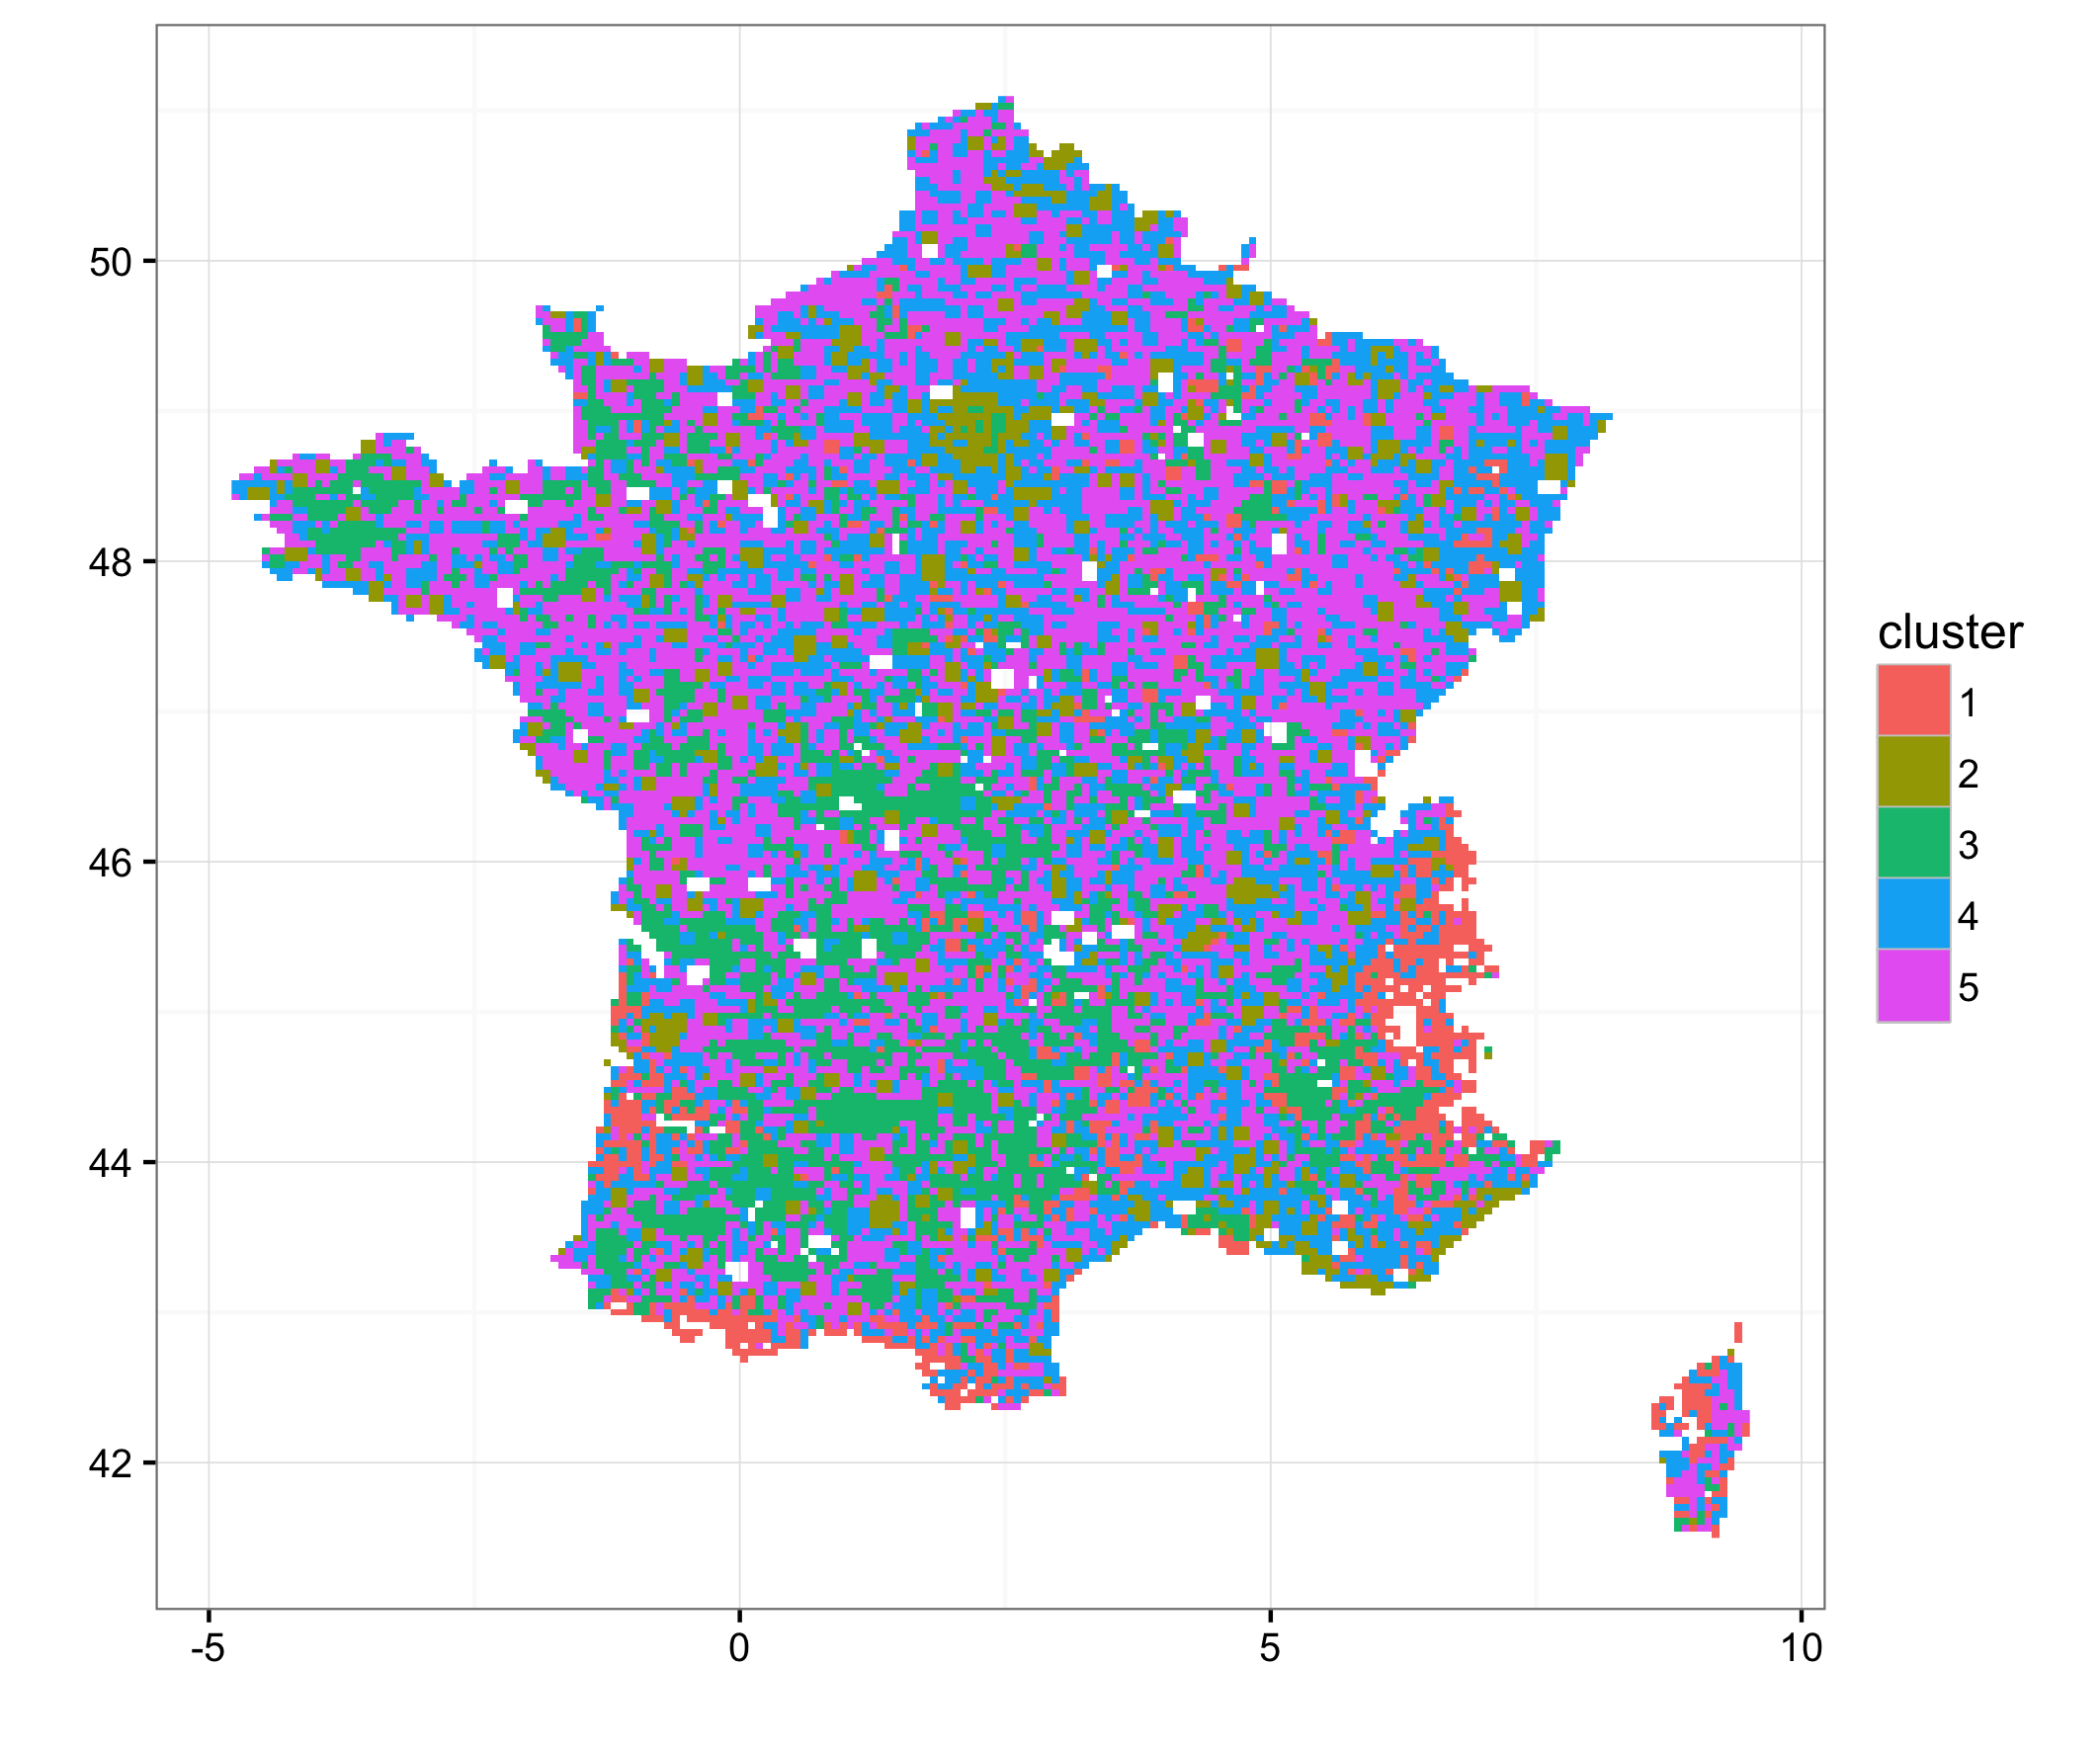
\includegraphics[width=\textwidth]{figures/density_cluster_map_k5_morpho}
\end{columns}

\justify

\footnotesize\textit{Computation of morphological indicators on population density data for Europe (shown here on France), morphological classification.}

}



\sframe{Population grids: model Calibration}{

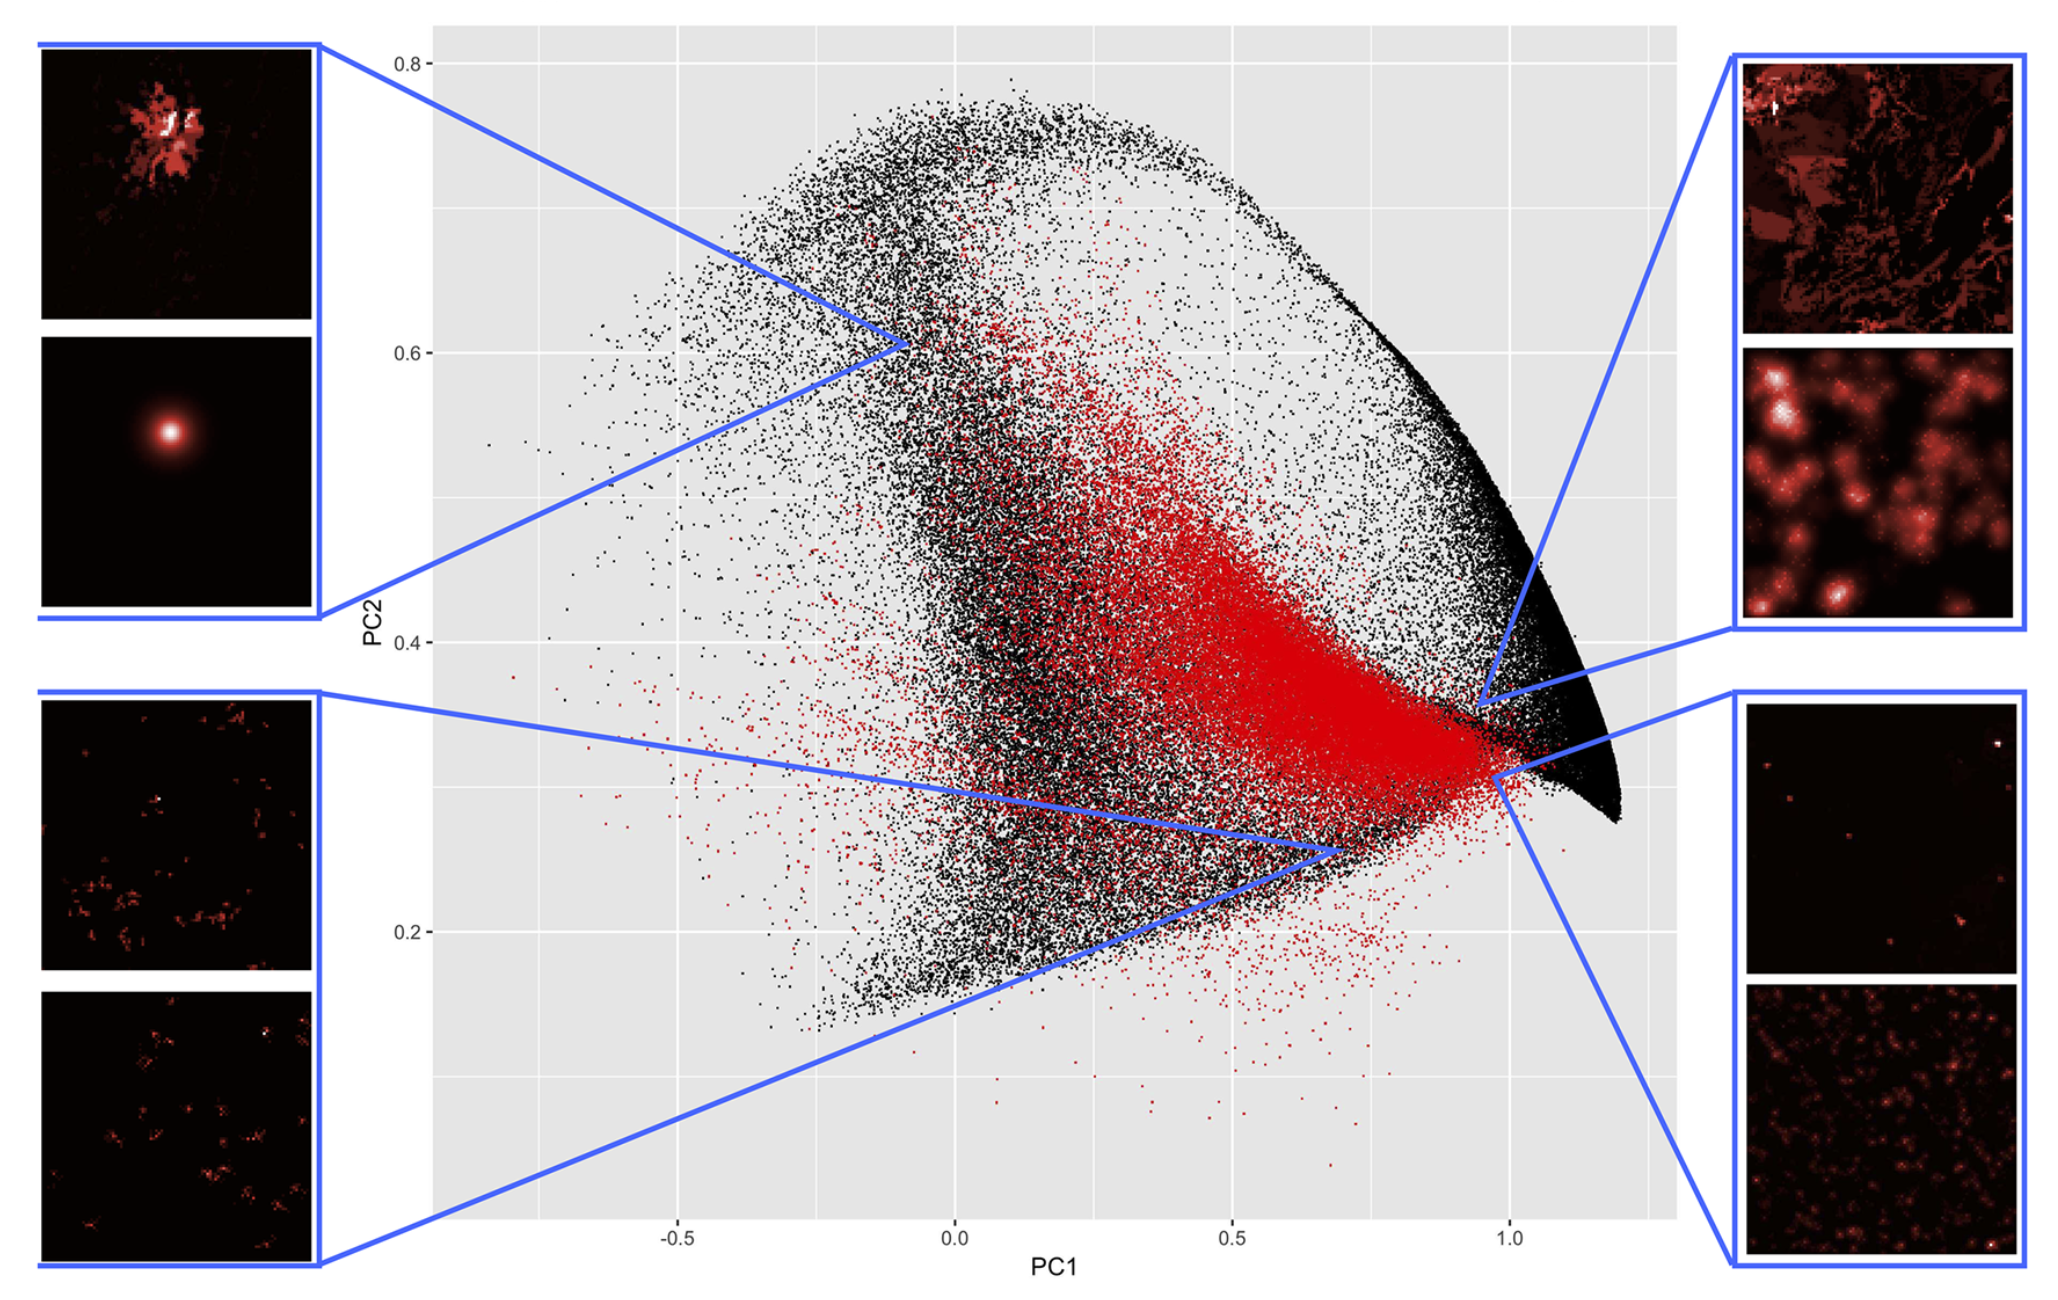
\includegraphics[width=\textwidth]{figures/spatialsens_calibmorphogenesis}

\footnotesize\textit{Brute force calibration by exploring the parameter space. Reproduction of most existing configuration in the morphological sense (here in principal plan).}

}









\subsection{Sensitivity to spatial configuration}



\sframe{Method flowchart}{

\textit{General workflow to test the spatial sensitivity of simulation models}

\bigskip

\footnotesize

Raimbault, J., Cottineau, C., Texier, M. L., Néchet, F. L., \& Reuillon, R. (2018). Space Matters: extending sensitivity analysis to initial spatial conditions in geosimulation models. arXiv preprint arXiv:1812.06008.

\bigskip

\centering

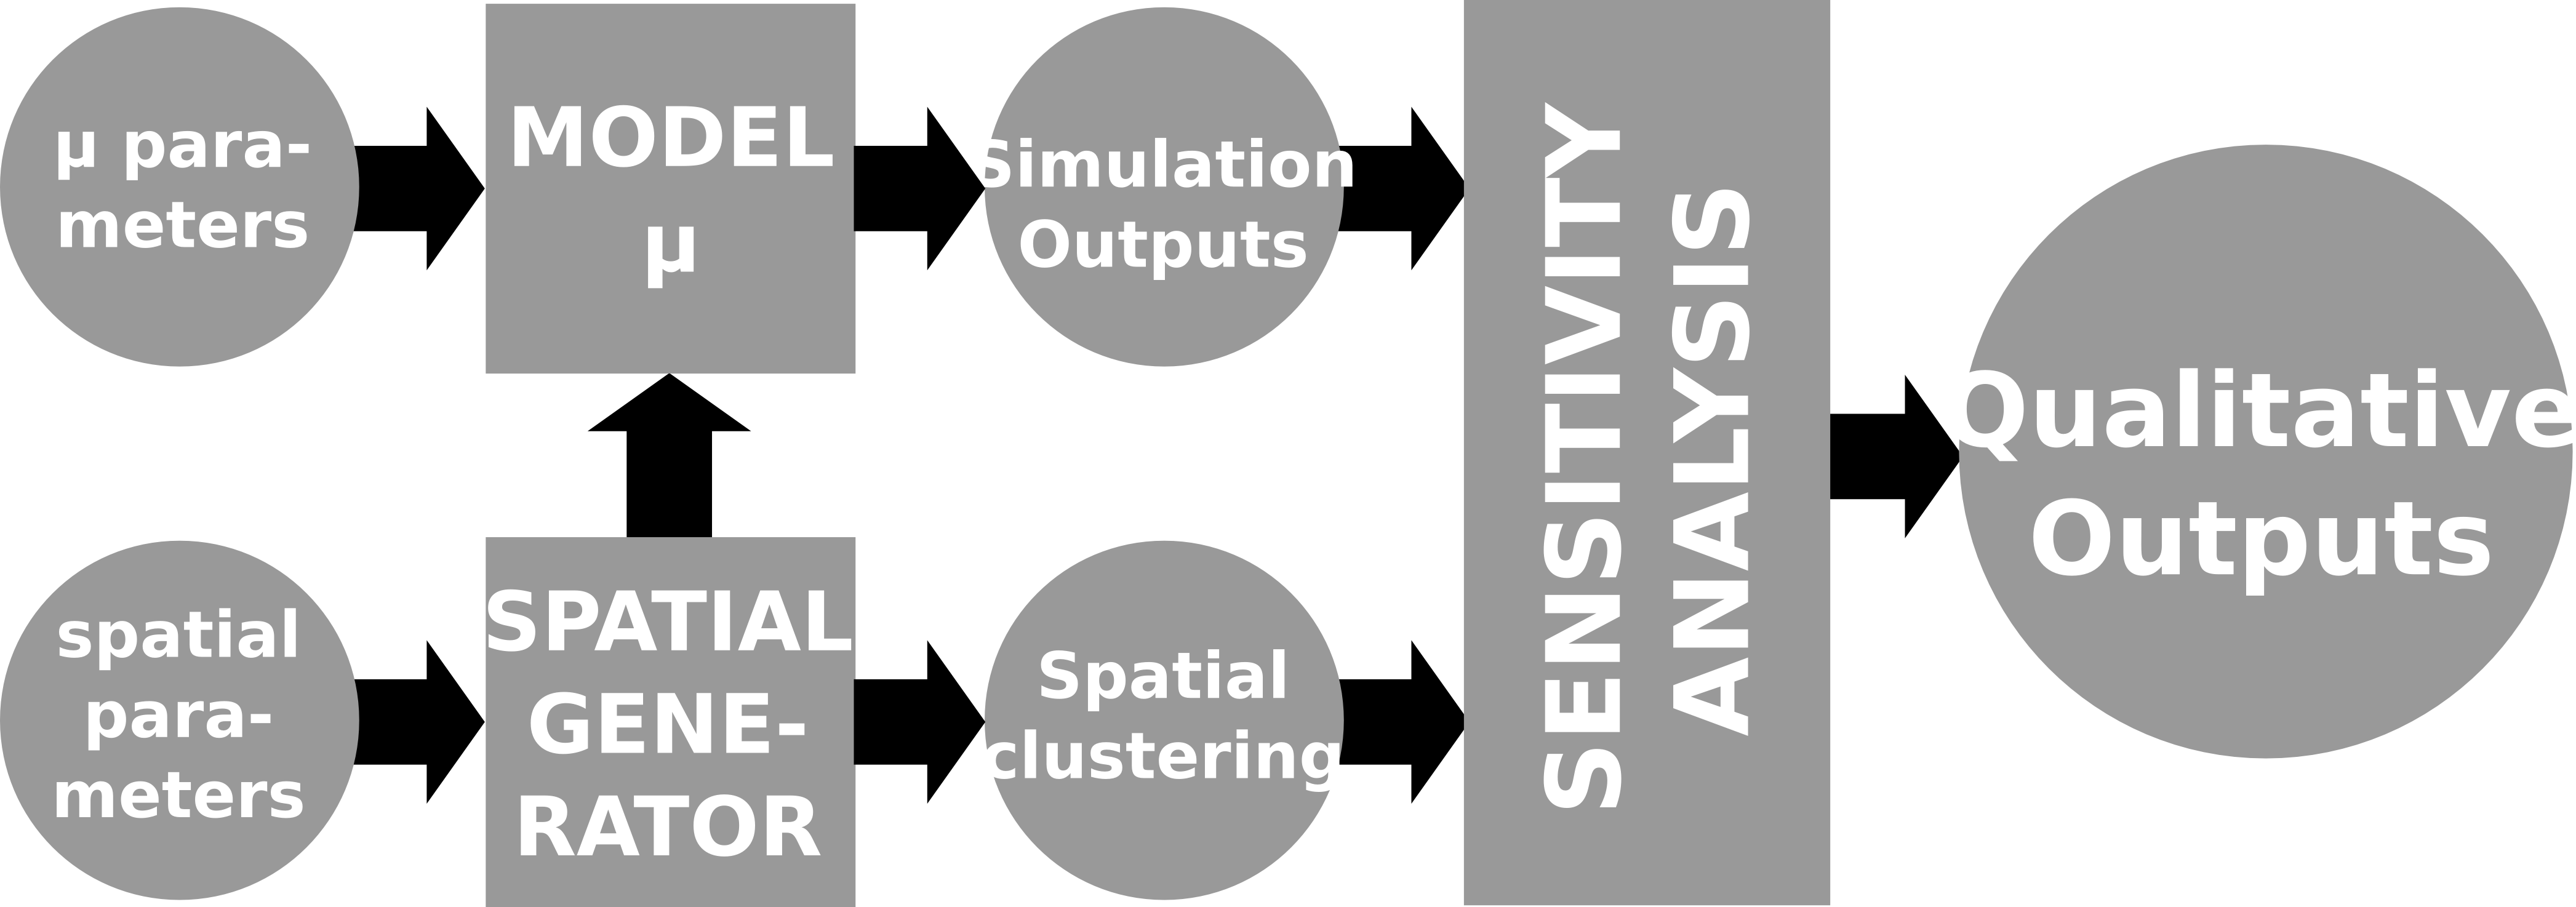
\includegraphics[width=\textwidth]{figures/spatialsens_spacemattersworkflow.png}

}


\sframe{Quantification of spatial sensitivity}{

\textit{Relative distance of phase diagrams to compare global model behavior when meta-parameters change}

\medskip

\[
d_r\left(\mu_{\vec{\alpha}_1},\mu_{\vec{\alpha}_2}\right) = 2 \cdot \frac{d(\mu_{\vec{\alpha}_1},\mu_{\vec{\alpha}_2})^2}{Var\left[\mu_{\vec{\alpha}_1}\right] + Var\left[\mu_{\vec{\alpha}_2}\right]}
\]

}


\sframe{Application: Schelling model}{

\textit{Why could the Schelling model be sensitive to space ?}

\medskip

\cite{banos2012network} network effects in Schelling model

\medskip

\centering

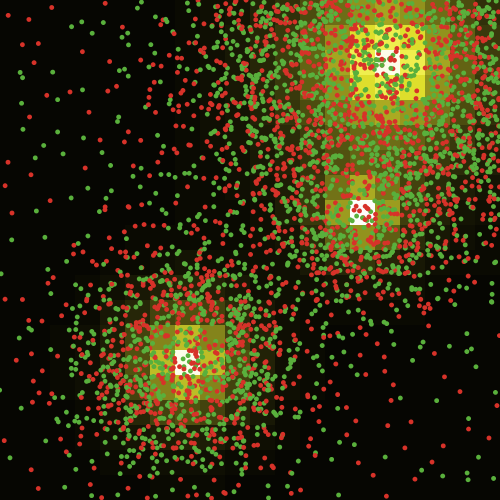
\includegraphics[width=0.45\textwidth]{figures/spatialsens_schelling_ex0_t0.png}
\hspace{0.1cm}
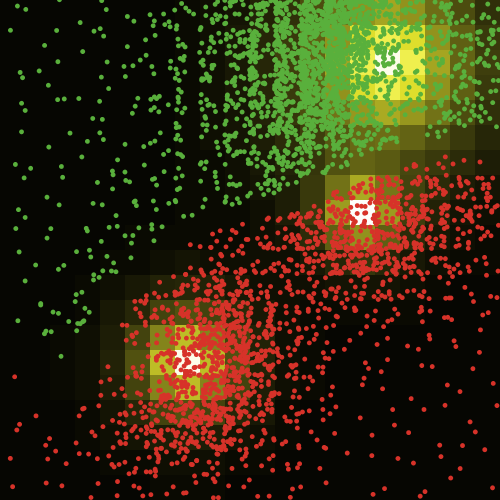
\includegraphics[width=0.45\textwidth]{figures/spatialsens_schelling_ex0_t91.png}


}


\sframe{Sensitivity of the Schelling model}{

\textit{Influence of spatial generator parameters on model outputs}

\centering

\includegraphics[height=0.8\textheight]{figures/spatialsens_schellingreg.png}

}


\sframe{Application: Sugarscape model}{

\textit{A model of resource collection}

\medskip

\begin{itemize}
	\item agents collect a spatial resource
	\item the resource regrows at a certain rate only
\end{itemize}


\bigskip


\textit{Relative distances between phase diagrams}

\medskip

\includegraphics[width=0.49\textwidth]{figures/sugarscape_Fig4.png}
\includegraphics[width=0.49\textwidth]{figures/sugarscape_Fig5.png}


}






\section{Discussion}




\sframe{Discussion}{

% morphogensis : interdisc ?

% suggest: ecology (habitat / spatial niches ?) ; topography ; ?

\textit{Spatial synthetic data in other disciplines ?}

\medskip

\begin{itemize}
	\item spatial network generative models
	\item other disciplines, ecology, geosciences \cite{mogheir2004characterizing}?
	\item interaction with data driven disciplines ? (planning, architecture, spatio-temporal datamining)
	\item genericity of some models ? (reaction-diffusion)
	\item synthetic data generation methods (synthetic populations)
	\item synthetic data at the core of applied statistics methodology (not much in spatial statistics ?)
\end{itemize}


}




\sframe{Synthesis of available tools}{



\begin{columns}
	\begin{column}{0.45\linewidth}
	
	\bigskip
	\bigskip
	
	Micro grid spatial samplings
	
	\medskip
	
	Meso grid spatial samplings
	
	\medskip
	
	Macro spatial samplings
	
	\medskip

	Spatial network generation
	
	\medskip

	Real data import
	
	\medskip

	Real data perturbations
	
	\medskip

	Spatial statistics
	
	\medskip

	Hybrid methods
	
	\medskip

	Domain models (transportation, land-use)
		
	\end{column}
	
	
	
	\begin{column}{0.2\linewidth}
		
		\vspace{-0.3cm}
		
		\textbf{OpenMOLE}
		
		\medskip
		
		{\textcolor{green}\cmark}
		
		\medskip
		
		{\textcolor{green}\cmark}
		
		\medskip
		
		{\textcolor{red}\xmark}
			
			\medskip
		
		{\textcolor{red}\xmark}
		
		\medskip
		
		{\textcolor{red}\xmark}
		
		\medskip
		
		{\textcolor{red}\xmark}
		
		\medskip

		{\textcolor{blue}\cmark}
		
		\medskip
		
		{\textcolor{red}\xmark}
		
		\medskip
		
		{\textcolor{red}\xmark}
			
	\end{column}
	
	
	
	\begin{column}{0.25\linewidth}
		
		\vspace{-0.3cm}
		
		\textbf{spatialdata}
		
		\medskip
		
		{\textcolor{green}\cmark}
		
		\medskip
		
		{\textcolor{green}\cmark}
		
		\medskip
		
		{\textcolor{green}\cmark}
			
			\medskip
		
		{\textcolor{blue}\cmark}
		
		\medskip
		
		{\textcolor{green}\xmark}
		
		\medskip
		
		{\textcolor{red}\xmark}
		
		\medskip

		{\textcolor{blue}\cmark}
		
		\medskip
		
		{\textcolor{red}\xmark}
		
		\medskip
		
		{\textcolor{blue}\cmark}
	\end{column}
	
	
	
	\begin{column}{0.2\linewidth}
		
		\vspace{-0.3cm}
		
		\textbf{planned}
		
		\medskip
		
		{\textcolor{green}\cmark}
		
		\medskip
		
		{\textcolor{green}\cmark}
		
		\medskip
		
		{\textcolor{green}\cmark}
			
			\medskip
		
		{\textcolor{green}\cmark}
		
		\medskip
		
		{\textcolor{green}\cmark}
		
		\medskip
		
		{\textcolor{green}\cmark}
		
		\medskip
		
		{\textcolor{green}\cmark}
		
		\medskip
		
		{\textcolor{green}\cmark}
		
		\medskip
		
		{\textcolor{green}\cmark}
	\end{column}

	
	
	
\end{columns}



}


\sframe{Conclusion}{

\justify

$\rightarrow$ \textbf{Space matters: } relevance of spatially-explicit models and spatial sensitivity analysis.

\bigskip

$\rightarrow$ \textbf{Synthetic data: } first experimental samplings included in OpenMOLE, soon more to come.

\bigskip

$\rightarrow$ \textbf{Disciplinary context: } strong contingency on included models and forms, please provide feedbacks, suggestions, needs, ideas from your viewpoint.

\medskip

\textit{Open issues at } \url{https://github.com/openmole/spatialdata/issues}

 

}






\backupbegin


%%%%%%%%%%%%%%%%%%%%%
\begin{frame}[allowframebreaks]
\frametitle{References}
\bibliographystyle{apalike}
\bibliography{biblio}
\end{frame}
%%%%%%%%%%%%%%%%%%%%%%%%%%%%


\backupend





\end{document}


